\documentclass[10pt,a4paper,twoside]{scrreprt}
\usepackage[english]{babel} 

\pagestyle{headings}

\addtolength{\voffset}{9mm}   %>>> moves text field down
\usepackage[latin1]{inputenc}   % Encodage ISO-8859-1.
\usepackage{graphicx}
\graphicspath{{images/}} 
\newcommand{\keyevidence}[1]{\fbox{#1}}

% Smaller italic font for marginpars
\let\oldmarginpar\marginpar
\renewcommand\marginpar[1]{\-\oldmarginpar[\raggedleft\footnotesize\it #1]%
{\raggedright\footnotesize\it #1}}

\usepackage{pgf}
\usepackage{hyperref}

\definecolor{webgreen}{rgb}{0,.5,0}
\definecolor{webbrown}{rgb}{.6,0,0}
\definecolor{Maroon}{cmyk}{0, 0.87, 0.68, 0.32}
\definecolor{RoyalBlue}{cmyk}{1, 0.50, 0, 0}

\usepackage{listings} 
\usepackage{makeidx}
\lstdefinelanguage{FIDOCAD} 
	{morekeywords={LI,PP,PV,TY,TE,MC,EV,EP,RP,RV,BE,SA,PA,PL,FCJ,FJC,CP,CV,%
		[FIDOCAD],[FIDOLIB]}, 
	sensitive=false, 
	morecomment=[s]{[}{]}, 
	morecomment=[s][\color{blue}]{\{}{\}}, 
	morecomment=[l][\color{violet}]{*},
	moredelim=[il][\color{violet}]{�},
} 

\lstset{language=FIDOCAD,%
	basicstyle=\small\ttfamily} 

% *******************************************************
% Hyperreferences
% *******************************************************
\hypersetup{%
    colorlinks=true, linktocpage=true, pdfstartpage=3, pdfstartview=FitV,%
    breaklinks=true, pdfpagemode=UseNone, pageanchor=true, pdfpagemode=UseOutlines,%
    plainpages=false, bookmarksnumbered, bookmarksopen=true, bookmarksopenlevel=1,%
    hypertexnames=true, pdfhighlight=/O,%hyperfootnotes=true,%nesting=true,%frenchlinks,%
    urlcolor=webbrown, linkcolor=RoyalBlue, citecolor=webgreen, %pagecolor=RoyalBlue,%
    % uncomment the following line if you want to have black links (e.g., for printing)
    %urlcolor=Black, linkcolor=Black, citecolor=Black, %pagecolor=Black,%
    pdftitle={FidoCadJ -- user manual},%
    pdfauthor={Davide Bucci},%
    pdfsubject={Comment utiliser FidoCadJ},%
    pdfkeywords={FidoCAD, FidoCadJ, CAD, electronics schematics, printed circuit boards},%
    pdfcreator={pdfLaTeX},%
    pdfproducer={LaTeX with hyperref and classicthesis}%
}
\lstset{frame=single,%
	backgroundcolor=\color{lightgray},
	keywordstyle=\color{RoyalBlue},
	breaklines=true
	}

\newcommand{\micron}{\,\mu\mathrm{m}}
\newcommand{\toprule}{\hline}

\newcommand{\midrule}{\hline}

\newcommand{\bottomrule}{\hline}

\title{\Huge\color{webbrown} FidoCadJ 0.24.1 \\ user manual} 


\author{Davide Bucci\\[3em]
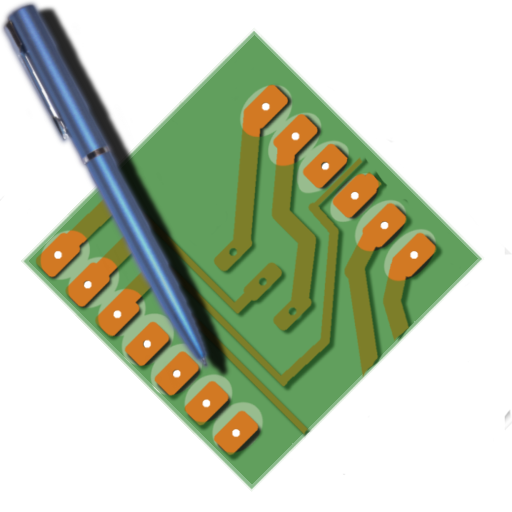
\includegraphics[width=.7\textwidth]{icona_fidocadj_a}
}

 \makeindex


\begin{document}
\pagenumbering{roman}

\pdfbookmark[1]{Front}{Front}
\maketitle 

\clearpage
\pdfbookmark[1]{Licence}{Licence}


\clearpage{} \pdfbookmark[1]{Licence}{Licence} This work is covered
by the Creative Commons Public License version 2.5 or more recent.
The entire text of this licence is available at the address\\
 \href{http://creativecommons.org/licenses/by-nc-nd/3.0/}{http://creativecommons.org/licenses/by-nc-nd/3.0/}.

You are free to reproduce, diffuse, communicate or expose in public,
represent, execute and play this work at the following conditions:
\begin{description}
\item [{Attribution}] {You must attribute the work in the manner specified
by the author or licensor (but not in any way that suggests that they
endorse you or your use of the work).} 
\item [{Noncommercial}] {You may not use this work for commercial purposes.} 
\item [{No Derivative Works}] {You may not alter, transform, or build
upon this work.} 
\end{description}
Any of the above conditions can be waived if you get permission from
the copyright holder (Davide Bucci). \vfill{}


All commercial names, logo, trademarks cited in this work are registered
by their owners.

\begingroup %\let\clearpage\relax
%\let\cleardoublepage\relax
%\let\cleardoublepage\relax



\chapter*{Abstract}

\pdfbookmark[1]{Abstract}{Abstract}

This document is the FidoCadJ official user manual. After a short
introduction of the history and the birth of this software, we will
describe the basic use of FidoCadJ. Our goal is to learn how to draw
very simple electronic schematics and their printed circuit boards.
The manual will end with a detailed description of the FidoCadJ (and
thus FidoCAD) format. Finally, we will give some hints about downloading and installing FidoCadJ using the most widespread operating systems: Linux, MacOSX and Windows.

\endgroup


\chapter*{Acknowledgements}

\pdfbookmark[1]{Aknowledgements}{Aknowledgements}

A number of people used this software from its first versions and
helped me by providing their advices. I thus want to thank the it.hobby.elettronica\index{it.hobby.elettronica}
newsgroup\index{newsgroup} participants for their very fruitful discussions.

This software has been very carefully tested on Linux thanks to
Stefano Martini's patience. He is a very attentive alpha and beta
tester! I would like to thank Olaf Marzocchi and Emanuele Baggetta
for their tests on MacOSX.

I would like to thank ``F. Bertolazzi'' who has given very useful
advices about the usability of this software. He also assembled the
CadSoft Eagle\index{Eagle} compatibility library, useful to export
FidoCadJ drawings to Eagle. Many thanks to ``Celsius'', who tested
the software functionalities for PCB realization, as well as its libraries.
Thanks to Andrea D'Amore, for his advice concerning FidoCadJ visual
aspect on the Apple Macintosh, from the 0.21.1 version. I would like to thank 
Roby IZ1CYN for the useful discussions about libraries and to have written 
section~\ref{installazione_linux} of this manual, about the Linux\index{Linux} 
installation.
Macintosh users can use FidoCadJ well integrated in the look of their operating system thanks to the Quaqua\index{Quaqua} look and feel, from Werner Randelshofer. 
Werner has given several useful advices about FidoCadJ's user interface: thanks!

This manual has been translated to English by ``Pasu''. I would like to thank him for his work. I would like to thank Miles ``qhg007'' as well, for the careful check and his very useful remarks.  

In April 2010, FidoCadJ has been integrated in the well known Italian web site \href{www.electroyou.it}{www.electroyou.it}. It silently runs on the server and it is used to automagically convert drawings posted by users of the forum.
I would like to express my gratitude to the admin Zeno Martini and webmaster Nicol� Martini and to all other users of this site as they gave me a lot of very useful ideas about batch controlling FidoCadJ: a very promising path has been traced which deserves to be fully explored. More recently, the FidoReadPHP class has been prepared in order to read and interpret FidoCadJ drawings on a PHP server. It has been used by the popular \href{www.grix.it}{www.grix.it}\index{www.grix.it} website thanks to Arniek and Sstrix. Kudos to them!

\chapter*{FidoCadJ License}

\pdfbookmark[1]{License FidoCadJ}{License FidoCadJ}

Copyright \copyright\ 2007-2012 Davide Bucci \href{mailto:davbucci@tiscali.it}{davbucci@tiscali.it}

This software is free: you can redistribute it and/or modify it under
the terms of the GNU General Public License as published by the Free
Software Foundation, version 3 of the License.

This program is distributed in the hope that it will be useful, but
WITHOUT ANY WARRANTY; without even the implied warranty of MERCHANTABILITY
or FITNESS FOR A PARTICULAR PURPOSE. See the GNU General Public License
for more details.

You should have received a copy of the GNU General Public License
along with this program. If not, see \href{http://www.gnu.org/licenses/}{http://www.gnu.org/licenses/}.

\tableofcontents
\pdfbookmark[1]{Table of contents}{Table of contents}

\listoffigures
\pdfbookmark[1]{Liste of figures}{List of figures}

\begingroup
\let\clearpage\relax
\let\cleardoublepage\relax
\let\cleardoublepage\relax
\listoftables
\pdfbookmark[1]{Liste of tables}{Liste of tables}

\endgroup

\chapter{Introduction} \pagenumbering{arabic} In this chapter,
we will briefly introduce FidoCadJ. In particular, we will give a
description of the philosophy behind this software, as well as a brief
history of its development.


\section{FidoCadJ's philosophy}

FidoCad\index{FidoCad} (without the J at the end) was a vectorial
drawing software particularly suit for electrical schematics\index{electrical schematic} as well
as printed circuit boards\index{PCB}. It is diffused in particular in the italian
Usenet community from late 1990s.

It can be freely downloaded (a Windows\index{Windows} version nationalized
in Italian language) from Lorenzo Lutti's page\index{Lorenzo Lutti}:

\href{http://www.enetsystems.com/~lorenzo/fidocad.asp}{http://www.enetsystems.com/\textasciitilde lorenzo/fidocad.asp}

The output files generated by this software is a very compact textual
description. This feature makes it very easy to include drawings in
text messages, such as those used in non binary Usenet groups\index{Usenet group}.

Unfortunately, FidoCad exists only in a Windows\index{Windows} version.
Who uses Linux can run it using WInE\index{WInE}, but for those using
other platforms like me (I use MacOSX) have to find a different solution.
I thus decided to give a small contribution to the Usenet community
by writing FidoCadJ (with the final J, this time). This editor is
written in pure Java\index{Java} and it is completely multi-platform.
FidoCadJ allows showing and modifying a drawing using the FidoCad\index{FidoCad}
file format.

Whoever used FidoCad\index{FidoCad} in the past should become acquainted
with FidoCadJ very quickly, since many commands and procedures are
quite similar to the original application. At the time of writing,
to the best of my knowledge, FidoCadJ is almost completely compatible
with the original FidoCad, apart from a few details. The goal of a complete compatibility has been pursued until possible, but recently the needs of the new users have pushed towards some extensions to the original format.

Among the features offered by FidoCadJ and not present in the original
FidoCad are the export possibilities offered. Since I am a \LaTeX{}
user, I decided to include an export feature for a number of vectorial
formats, including Encapsulated PostScript (\textsc{EPS}\index{EPS}). Of course, FidoCadJ can export towards the very well known \textsc{PDF}\index{PDF} format.
Another file format useful for electronic schematics is the CadSoft
Eagle script\index{CadSoft Eagle}, which is available from version
0.21 of FidoCadJ. In this way, a schematics drawn with FidoCadJ can
be exported to Eagle.
The appendix~\ref{specifics} briefly describes how to install FidoCadJ on 
the most diffused operating systems.


\section{History of this software}

I have long been interested in electronic circuits. When I began following
several dedicated italian Usenet newsgroups\index{newsgroups}, I
noticed that many schematics were provided using the FidoCad for Windows
format\index{FidoCad}. This avoided awkward ASCII drawings. Since
I do not use Windows since a few years ago, it was almost impossible
for me to look at them and I wanted to try to do something to solve
this problem. \marginpar{By the way, I think that it is better to
work at a solution rather claim that an operating system different
from Windows lacks in software}

The first thing I did was to study the file format used by FidoCad\index{FidoCad}
and write a Java\index{Java} applet called FidoReadJ\index{FidoReadJ},
able to parse the circuit and to show it in a web page. I started
searching more or less everywhere (old posts, web pages), doing a
lot of reverse engineering from existing FidoCad files. I downloaded
the FidoCad sources, written in a pretty neat C++ by Lorenzo Lutti.

I did this work more or less around March 2007. A few moths later,
the applet was on line and it was being tested by part of the community
gravitating around it.hobby.elettronica\index{it.hobby.elettronica}
and it.hobby.fai-da-te\index{it.hobby.fai-da-te}.%
\footnote{FidoReadJ\index{FidoReadJ} is still available at the address:\\
 \href{http://davbucci.chez-alice.fr/index.php?argument=elettronica/fidoreadj/fidoreadj.inc\&language=Francais}{http://davbucci.chez-alice.fr/index.php?argument=elettronica/fidoreadj/fidoreadj.inc}.%
}

Since I had an interpreter\index{interpreter} of the FidoCad format,
it was interesting to continue the work in order to obtain a complete
editor\marginpar{To be honest, I made a first attempt at writing
a 2D vectorial drawing system around 1993.} The most part of the
work was done in several steps, between January and July 2008. FidoCadJ
is not an adaptation or a porting of FidoCad for Windows, but it is
a completely rewritten program.

The choice of using Java\index{Java} is due to the fact that in the
last few years I changed a lot of operating systems. Spending time
and energies on something which is not completely portable does not
appeal to me anymore. The effort of learning the Cocoa framework would
have probably given a better result on MacOSX, but it would have
made FidoCadJ completely non-portable. I am not a computer guy. The
time I spend to program is time taken away from my electronics interests.
In fact, a simple analysis of the FidoCadJ code source shows that
I am not a very Java\index{Java} and object oriented programming\index{Object oriented programming}
purist and I am sure that several solutions could be found that are
more practical than elegant.

What matters is the end user impressions while using the program,
more than the choice of a particular language. For this reason, I
am always listening to your suggestions, in order to understand how
to further develop this project. To summarize, I am aware that Java\index{Java}
is not the perfect choice or the solution to every problem. However
I am sure that its bad name derives mostly from badly written applications
which are not very well integrated with the user desktop.

% La parte interamente tradotta da Pasu comincia qui.


Without aiming for perfection and knowing my programming skills limitations,
my intent is to make sure that FidoCadJ will NOT be another poor quality
application. For this reason any bug report or comment on the program's
usability will be more than welcome.

Since november 2009, I opened a SourceForge\index{SourceForge} project dedicated to FidoCadJ. 
From this page, you can download all executables, manuals as well as the source
code. You can actively participate to FidoCadJ development working on the 
source code using Subversion (SVN), or the SVN browser provided by SourceForge:

�\href{http://fidocadj.svn.sourceforge.net/viewvc/fidocadj/}{http://fidocadj.svn.sourceforge.net/viewvc/fidocadj/} 

If you want to help me with FidoCadJ, do not worry: you do not need to be an
expert Java programmer. You can for example translate the user interface or the 
manuals in a new language, check carefully the existing manuals for inconsistencies and
errors. You can also work on the standard library\dots\
Consider that only the half of the spare time I dedicate to FidoCadJ is in reality dedicated to the coding activity. The rest is spent answering questions from users, writing and improving the documentation and so on.
On SourceForge\index{SourceForge}, you can participate to the forums, write a 
program review as well as suggest improvements or give a bug report:

\href{http://sourceforge.net/projects/fidocadj/}{http://sourceforge.net/projects/fidocadj/}

\section{FidoCadJ and the future}

In april 2010, I stumbled almost accidentally on a thread in a well known italian website \href{www.electroyou.it}{www.electroyou.it}. An user, Giancarlo Boletti, proposed to integrate a schematic capture tool directly inside the forum. Something similar has already been done with \LaTeX\index{LaTeX@\LaTeX} equations. Since FidoCadJ was cited in his intervention, I inscribed myself to the forum and I offered to collaborate. I interacted with the very nice webmaster for a few days, and then the system was ready: a simple copy and paste in a post of the code describing the drawing, with a couple of tags. The forum software runs FidoCadJ on its servers and obtains an image, directly from the code. This image is then shown in the forum post, but its source code remains available. This way, who is reading the discussion does not need to have anything installed, but if he desires to change something, he can obtain the code with a few clicks.

Figure~\ref{fig_discussione_electroyou} shows part of one of my posts done on  \href{www.electroyou.it}{www.electroyou.it}. This system is so powerful and flexible that I have been the first to be astonished of the enthusiasm demonstrated by the users!\footnote{If you read Italian, here is an article I wrote:\\ \href{http://www.electroyou.it/darwinne/wiki/fidocadj}{http://www.electroyou.it/darwinne/wiki/fidocadj}	 }
 	 
\begin{figure}
 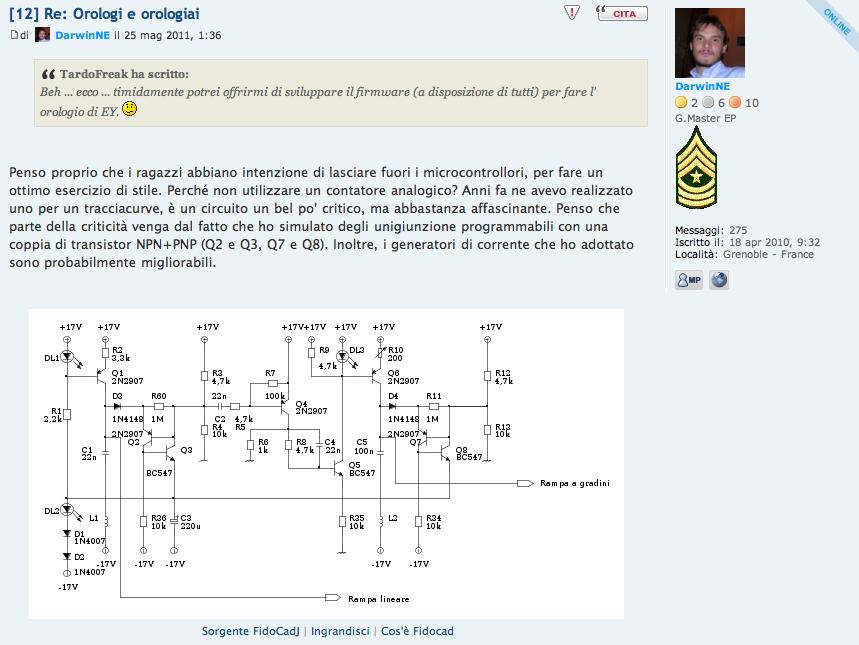
\includegraphics[width=\textwidth]{discussione_electroyou.png}
 \caption{Part of one of my posts on \href{www.electroyou.it}{www.electroyou.it}\index{www.electroyou.it}.
 With just one click you can zoom on the schematic. With a second one, you can obtain immediately the source code that you can paste on FidoCadJ to modify it.}
\label{fig_discussione_electroyou}
\end{figure}


The success that FidoCadJ has had on \href{www.electroyou.it}{www.electroyou.it}\index{www.electroyou.it} has stimulated some requests to implement a similar system on other platforms, and in particular on \href{www.electroyou.it}{www.electroyou.it}\index{www.electroyou.it}, another well known Italian electronics-dedicated website.
In this case, the server could not run a Java program and so the FidoReadPHP class has been written. It can be run on a PHP interpreter to obtain the images from the FidoCadJ source code.
The FidoReadPHP project is open source and it is available on SourceForge:

\href{https://sourceforge.net/projects/fidoreadphp/}{https://sourceforge.net/projects/fidoreadphp/}

The result is somewhat similar to what it has been obtained on \href{www.electroyou.it}{www.electroyou.it}, even if the graphical capabilities of PHP are quite limited in comparison with Java.
\footnote{Once again, if you read Italian, here is an article:\\
\href{http://www.grix.it/viewer.php?page=9335}{http://www.grix.it/viewer.php?page=9335}}
Figure~\ref{fig_fidocadj_grix3} shows an example of a drawing obtained with FidoReadPHP.

\begin{figure}
 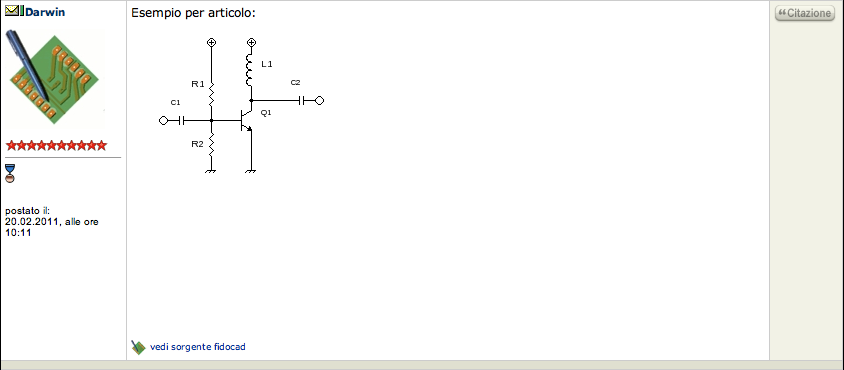
\includegraphics[width=\textwidth]{fidocadj_grix3.png}
 \caption{An example of a FidoCadJ drawing integrated in a \href{www.grix.it}{www.grix.it}\index{www.grix.it} forum post. You can obtain the source code of the drawing with just a mouse click.}
 \label{fig_fidocadj_grix3}
\end{figure}

I think that the future of FidoCadJ is not to become more complex, as a complete CAD for electronics. Probably, those possibilities of integration with discussion groups and forums deserve to be developed. Experience has shown that this is possible and the enthusiasm of the users has been tantalizing. 

\chapter{Drawing with FidoCadJ}

The use of FidoCadJ should be quite intuitive for those who already
used a vectorial drawing application\index{vectorial drawing}. A
screenshot of the program running on MacOSX\index{MacOSX} is shown
in Fig.~\ref{fig_fidocadj};\marginpar{Expert Mac-users will notice
that all the menus are at their own place!} A few details may be
different when running on other operating systems (for example
Fig.~\ref{fig_metal} shows the result with Look and Feel Metal\index{Metal}
on Sun/Oracle\index{Sun/Oracle}), but the philosophy remains the same. We will
see what the features of the program are, and its basic elements (the
primitives)\index{primitive} which compose a FidoCadJ drawing. %
\begin{figure}
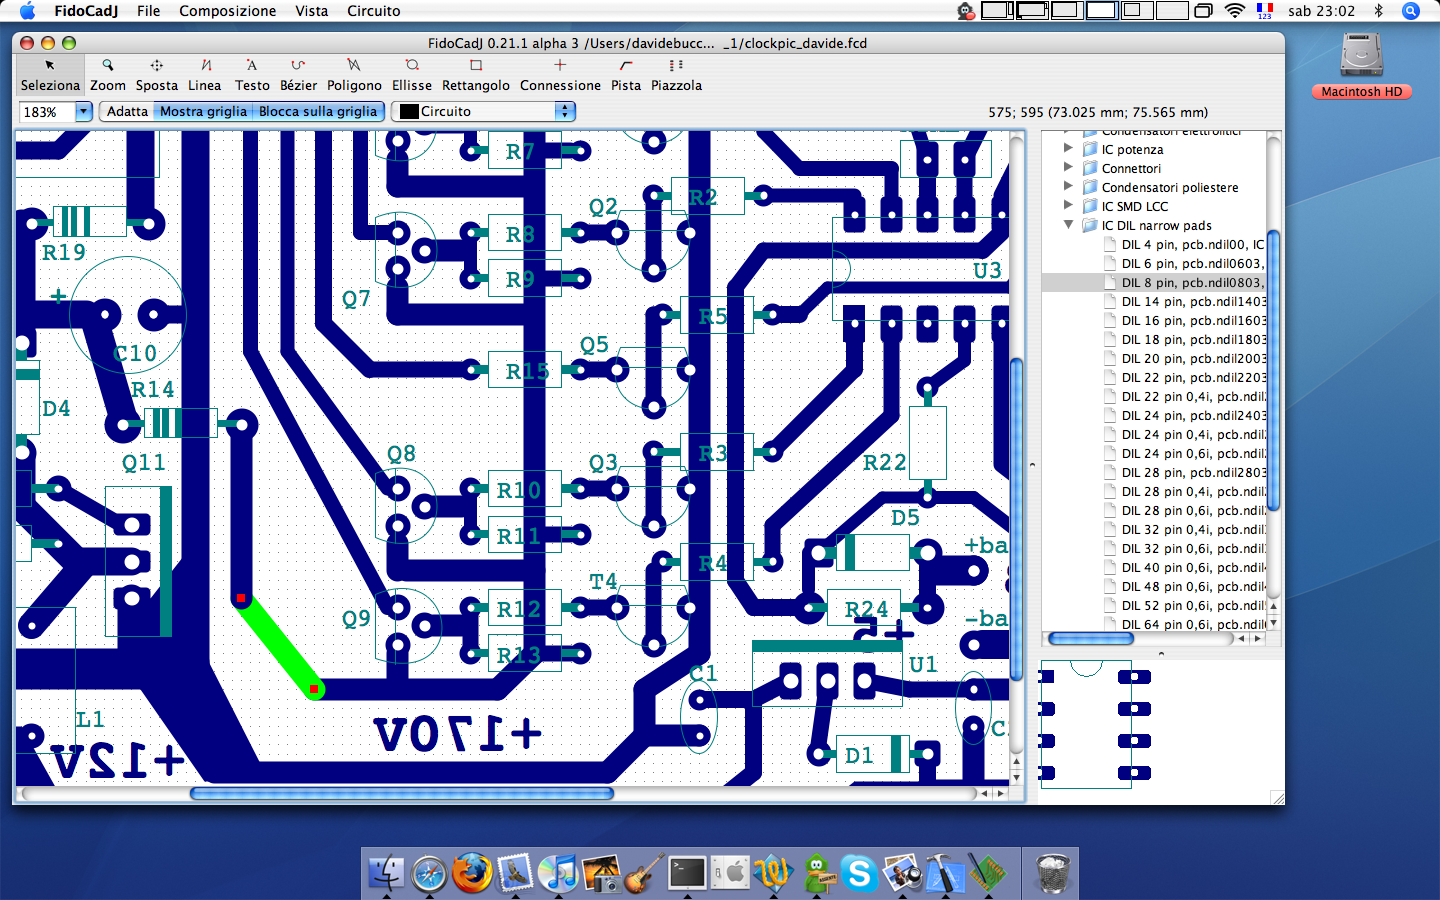
\includegraphics[width=1\textwidth]{fidocadj_macosx.png} 

\caption{A typical FidoCadJ session running on MacOSX Tiger\index{MacOSX}.
Appendix~\ref{specifics} describes the peculiarities of the version
specific for Macintosh\index{Macintosh}.}


\label{fig_fidocadj} 
\end{figure}


%
\begin{figure}
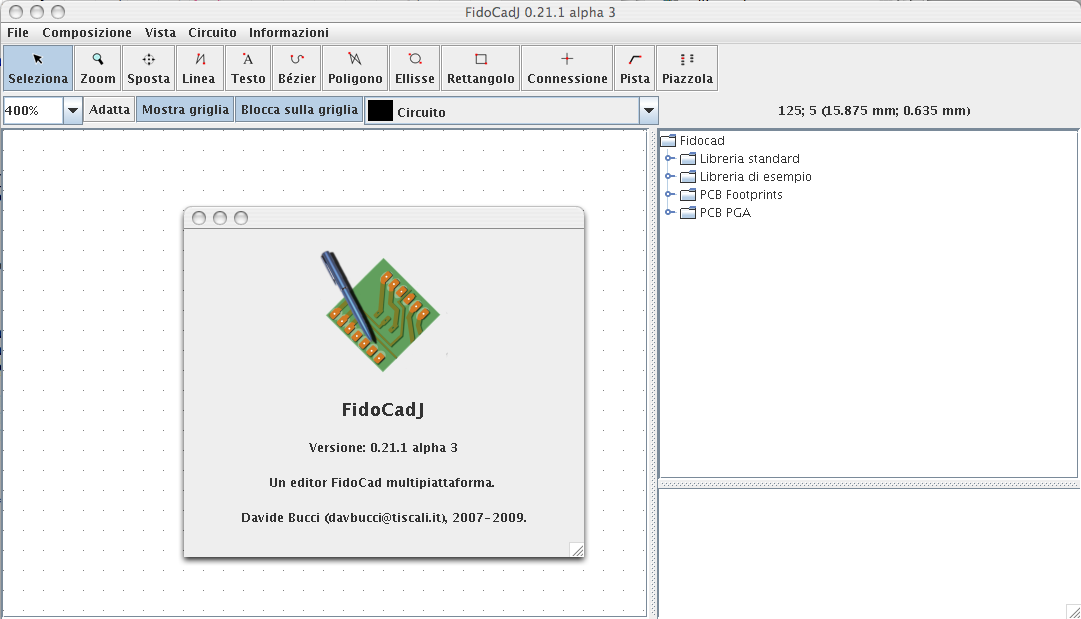
\includegraphics[width=1\textwidth]{fidocadj_metal.png} 

\caption{FidoCadJ with the Look and Feel Metal\index{Metal}.}


\label{fig_metal} 
\end{figure}



\section{Drawing Tools}

In the toolbar\index{toolbar} (on the top of the window), we can
find the most used features that allow the creation and the editing
of a drawing. Table~\ref{tab_comandi} shows a brief summary of the
functionalities and the commands and describes the possible actions.
You will notice that once a button is pressed, it will remain in that
position until another function from the toolbar will be selected.\marginpar{This
behavior is inspired to the old vacuum tube radios and to the switches
very fashionable in the '70s.} From the toolbar we can select which
drawing primitive\index{primitive} will be used.%
\footnote{For more information on the drawing elements, see~\ref{sec_primitive}.%
} On the right, a drop-down menu will show the current working layer
(see~\ref{sec_layer} for more information).

The command bar\index{command bar} can be partially customized. In
particular, we can choose whether we want to see the icon on each
button or the icon and its text description. Icons are also available
in two selectable formats. To change these settings we can select
the menu {}``File/Options''.%
\footnote{Except on MacOSX, where this item is found in the FidoCadJ's menu
and it is called {}``Preferences''.%
} Any change in the settings will be applied at the restart of the
application, since it is arguably something that we may want to change
every day. Figures \ref{fig_fidocadj} and \ref{fig_metal} show the
command bar (right below the window's title), configured to show text
and icons in their smallest version. On the second row, starting from
the left we can see the zoom settings and the buttons {}``Fit'',
{}``Show grid'' e {}``Snap to grid''. The first allows us to automatically
select the most suitable zoom settings in order to show the whole
drawing on the screen. The second toggles between visible and invisible
grid, while when we press the third button the elements added will
stick to the nearest step of the grid.
If you need to align carefully the elements, you may find useful to keep pressed \keyevidence{Alt}, while using the cursor keys.

%
\begin{table}
\centering \begin{tabular}{clp{0.5\textwidth}}
\toprule Key & Comando  & Use\tabularnewline
\midrule

\keyevidence{A} or \keyevidence{Spacebar} & \raisebox{-.2em}{
\includegraphics[width=1em]{icons/arrow}}
\textsc{Select}\index{selection}  & Selects one or more graphic elements. Press \keyevidence{Control}
(\keyevidence{Command} only on MacOSX) for multiple selections
or to deselect only one element. Click and drag to select several
elements in an area. Press \keyevidence{R} to rotate the selected
elements. Press \keyevidence{S} to mirror the selected elements.
Double-click on an element to modify its properties.\tabularnewline
 & \raisebox{-.2em}{
\includegraphics[width=1em,]{icons/magnifier}}
\textsc{Zoom}\index{zoom}  & Left-click to increase the level of zoom. Right-click to decrease
it.\tabularnewline
 & \raisebox{-.2em}{
\includegraphics[width=1em,]{icons/move}}
\textsc{Move}\index{move}  & Click on the drawing and move the mouse to move the drawing.\tabularnewline
\keyevidence{L}  & \raisebox{-.2em}{
\includegraphics[width=1em,]{icons/line}}
\textsc{Line}\index{line}  & Inserts a line or a series of lines. Press \keyevidence{Esc} or
double-click to terminate the insertion %\footnote{In FidoCadJ versions prior to 0.20.5, a right click would switch to the ``Select'' mode}
\tabularnewline
\keyevidence{T}  & \raisebox{-.2em}{
\includegraphics[width=1em,]{icons/text}}
\textsc{Text}\index{text}  & Inserts a text string.\tabularnewline
\keyevidence{B}  & \raisebox{-.2em}{
\includegraphics[width=1em,]{icons/bezier}}
\textsc{B�zier}\index{B�zier}  & Draws a B�zier curve\tabularnewline
\keyevidence{P}  & \raisebox{-.2em}{
\includegraphics[width=1em,]{icons/polygon}}
\textsc{Polyline}\index{polyline}  & Draws a polyline filled or empty. Double-click or press \keyevidence{Esc},
to terminate the insertion of new vertices.\tabularnewline
\keyevidence{K}
&
\raisebox{-.2em}{%

\includegraphics[width=1em]{icons/complexcurve}%
}
\textsc{Curve}\index{curve}
&
Open or closed natural cubic spline curve. Double click or press \keyevidence{Esc},  to terminate the insertion of new vertices.\tabularnewline

\keyevidence{E}  & \raisebox{-.2em}{
\includegraphics[width=1em,]{icons/ellipse}}
\textsc{Ellipse}\index{ellipse}  & Draws an ellipse filled or empty (hold \keyevidence{Control} to
draw a circle). \tabularnewline
\keyevidence{G}  & \raisebox{-.2em}{
\includegraphics[width=1em,]{icons/rectangle}}
\textsc{Rect.}\index{rectangle}  & Draws a rectangle filled or empty.\tabularnewline
\keyevidence{C}  & \raisebox{-.2em}{
\includegraphics[width=1em,]{icons/connection}}
\textsc{Junction}\index{junction}  & Inserts an electrical junction.\tabularnewline
\keyevidence{I}  & \raisebox{-.2em}{
\includegraphics[width=1em,]{icons/pcbline}}
\textsc{PCB track}\index{PCB track}  & Draws a PCB track. The default width can be modified through the dialog
accessed from the menu {}``File/Options''. \tabularnewline
\keyevidence{Z}  & \raisebox{-.2em}{
\includegraphics[width=1em,]{icons/pcbpad}}
\textsc{PCB pad}\index{PCB pad@\textsc{PCB }pad}  & Draws a PCB pad. The default dimensions can be modified through the
dialog accessed from the menu {}``File/Options''. \tabularnewline
\bottomrule  &  & \tabularnewline
\end{tabular}

\caption{Summary of the drawing commands available in FidoCadJ. The key shown
on the leftmost column allows their rapid selection using the keyboard.
A right click in one of the primitive placement modes allows us to
access the properties window.}


\label{tab_comandi} 
\end{table}


On the right are shown in a tree list the elements \index{macro}
(called macro) of the libraries loaded into the application. To insert
an element from the library we only need to select it from the list
an click on the drawing. FidoCad\index{FidoCad} libraries include
all standard symbols used in electrical schematics\index{electrical schematic} and a wide selection of footprints\index{PCB!footprint} for drawing PCBs.

From version 0.22, you can do quick research\index{Quick research} inside the libraries charged in FidoCadJ. You just need to type something in the text field which appears just over the tree representing the installed libraries (have a look to figure~\ref{fig_ricerca}) 
By typing up and down keys, you can navigate through the results found.

\begin{figure}
\centering
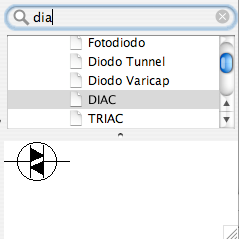
\includegraphics[width=.4\textwidth]{ricerca}
\caption{The quick search function in the installed libraries.}
\label{fig_ricerca}
\end{figure}
%
\begin{figure}
\centering 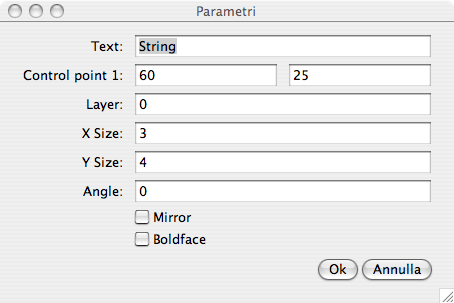
\includegraphics[width=0.7\textwidth,]{param_testo} 

\caption{Dialog for the text's parameters in a FidoCadJ drawing.}


\label{fig_param_testo} 
\end{figure}


Figure~\ref{fig_param_testo} shows an example of what we can obtain
by double-clicking, in selection mode\index{selection}, on a drawing
element (in this case a text string). Within this window it is possible
to modify all the parameters (coordinates, rotation\dots) of any
drawing element. The aspect of this window will change because the
information that can be modified will depend on the selected element.


\section{A simple schematic}

As an example of use of this application, we will show how to draw
the simple electrical schematic of figure~\ref{fig_schema}. %
\begin{figure}
\centering %\includegraphics[width=.5\textwidth]{schema}
\begin{pgfpicture}{0cm}{0cm}{125pt}{111pt}
% Created by FidoCadJ ver. 0.21, export filter by Davide Bucci
\pgfsetxvec{\pgfpoint{1pt}{0pt}}
\pgfsetyvec{\pgfpoint{0pt}{1pt}}
\pgfsetlinewidth{0.33pt}
\pgfsetroundjoin 
\pgftranslateto{\pgfxy(0,111)}
\begin{pgfmagnify}{1}{-1}
% Layer color definitions
\definecolor{layer0}{rgb}{0.0,0.0,0.0}
\definecolor{layer1}{rgb}{0.0,0.0,0.5}
\definecolor{layer2}{rgb}{1.0,0.0,0.0}
\definecolor{layer3}{rgb}{0.0,0.5,0.5}
\definecolor{layer4}{rgb}{1.0,0.78,0.0}
\definecolor{layer5}{rgb}{1.0,0.78,0.0}
\definecolor{layer6}{rgb}{1.0,0.78,0.0}
\definecolor{layer7}{rgb}{1.0,0.78,0.0}
\definecolor{layer8}{rgb}{1.0,0.78,0.0}
\definecolor{layer9}{rgb}{1.0,0.78,0.0}
\definecolor{layer10}{rgb}{1.0,0.78,0.0}
\definecolor{layer11}{rgb}{1.0,0.78,0.0}
\definecolor{layer12}{rgb}{1.0,0.78,0.0}
\definecolor{layer13}{rgb}{1.0,0.78,0.0}
\definecolor{layer14}{rgb}{1.0,0.78,0.0}
\definecolor{layer15}{rgb}{1.0,0.78,0.0}
% End of color definitions
\color{layer0}
\pgfline{\pgfxy(100,67)}{\pgfxy(105,70)}
\pgfline{\pgfxy(90,65)}{\pgfxy(100,65)}
\pgfline{\pgfxy(100,60)}{\pgfxy(100,70)}
\pgfline{\pgfxy(105,60)}{\pgfxy(105,55)}
\pgfline{\pgfxy(100,63)}{\pgfxy(105,60)}
\pgfline{\pgfxy(105,70)}{\pgfxy(105,75)}
\pgfmoveto{\pgfxy(103,70)}
\pgflineto{\pgfxy(104,68)}
\pgflineto{\pgfxy(105,70)}
\pgfclosepath 
\pgffill 
\begin{pgfmagnify}{1}{-1}
\pgfputat{\pgfxy(110,-55)}{\pgfbox[left,top]{\footnotesize{Q1B}}}
\end{pgfmagnify}
\begin{pgfmagnify}{1}{-1}
\pgfputat{\pgfxy(110,-65)}{\pgfbox[left,top]{\footnotesize{LM394}}}
\end{pgfmagnify}
\pgfline{\pgfxy(40,67)}{\pgfxy(35,70)}
\pgfline{\pgfxy(50,65)}{\pgfxy(40,65)}
\pgfline{\pgfxy(40,60)}{\pgfxy(40,70)}
\pgfline{\pgfxy(35,60)}{\pgfxy(35,55)}
\pgfline{\pgfxy(40,63)}{\pgfxy(35,60)}
\pgfline{\pgfxy(35,70)}{\pgfxy(35,75)}
\pgfmoveto{\pgfxy(37,70)}
\pgflineto{\pgfxy(36,68)}
\pgflineto{\pgfxy(35,70)}
\pgfclosepath 
\pgffill 
\begin{pgfmagnify}{1}{-1}
\pgfputat{\pgfxy(10,-55)}{\pgfbox[left,top]{\footnotesize{Q1A}}}
\end{pgfmagnify}
\begin{pgfmagnify}{1}{-1}
\pgfputat{\pgfxy(0,-65)}{\pgfbox[left,top]{\footnotesize{LM394}}}
\end{pgfmagnify}
\pgfline{\pgfxy(50,65)}{\pgfxy(90,65)}
\pgfline{\pgfxy(35,75)}{\pgfxy(35,95)}
\pgfline{\pgfxy(105,75)}{\pgfxy(105,95)}
\pgfline{\pgfxy(35,40)}{\pgfxy(35,55)}
\pgfline{\pgfxy(35,30)}{\pgfxy(35,32)}
\pgfmoveto{\pgfxy(36,32)}
\pgflineto{\pgfxy(34,32)}
\pgflineto{\pgfxy(34,38)}
\pgflineto{\pgfxy(36,38)}
\pgfclosepath 
\pgfqstroke 
\pgfline{\pgfxy(35,38)}{\pgfxy(35,40)}
\begin{pgfmagnify}{1}{-1}
\pgfputat{\pgfxy(45,-40)}{\pgfbox[left,top]{}}
\end{pgfmagnify}
\begin{pgfmagnify}{1}{-1}
\pgfputat{\pgfxy(45,-35)}{\pgfbox[left,top]{}}
\end{pgfmagnify}
\pgfline{\pgfxy(35,15)}{\pgfxy(35,30)}
\pgfline{\pgfxy(25,15)}{\pgfxy(35,15)}
\pgfline{\pgfxy(25,15)}{\pgfxy(23,15)}
\pgfellipse[stroke]{\pgfxy(21.0,15.0)}{\pgfxy(2.0,0)}{\pgfxy(0,2.0)}
\pgfline{\pgfxy(22,15)}{\pgfxy(20,15)}
\pgfline{\pgfxy(21,16)}{\pgfxy(21,14)}
\begin{pgfmagnify}{1}{-1}
\pgfputat{\pgfxy(35,-25)}{\pgfbox[left,top]{}}
\end{pgfmagnify}
\begin{pgfmagnify}{1}{-1}
\pgfputat{\pgfxy(35,-20)}{\pgfbox[left,top]{}}
\end{pgfmagnify}
\pgfline{\pgfxy(35,50)}{\pgfxy(55,50)}
\pgfline{\pgfxy(55,50)}{\pgfxy(55,65)}
\pgfcircle[fill]{\pgfxy(55,65)}{1pt}\pgfcircle[fill]{\pgfxy(35,50)}{1pt}\pgfline{\pgfxy(105,45)}{\pgfxy(105,55)}
\pgfline{\pgfxy(105,35)}{\pgfxy(105,40)}
\pgfline{\pgfxy(105,25)}{\pgfxy(105,30)}
\pgfline{\pgfxy(35,95)}{\pgfxy(35,100)}
\pgfline{\pgfxy(32,100)}{\pgfxy(38,100)}
\pgfline{\pgfxy(33,101)}{\pgfxy(37,101)}
\pgfline{\pgfxy(34,102)}{\pgfxy(36,102)}
\begin{pgfmagnify}{1}{-1}
\pgfputat{\pgfxy(45,-105)}{\pgfbox[left,top]{}}
\end{pgfmagnify}
\begin{pgfmagnify}{1}{-1}
\pgfputat{\pgfxy(45,-100)}{\pgfbox[left,top]{}}
\end{pgfmagnify}
\pgfline{\pgfxy(105,95)}{\pgfxy(105,100)}
\pgfline{\pgfxy(102,100)}{\pgfxy(108,100)}
\pgfline{\pgfxy(103,101)}{\pgfxy(107,101)}
\pgfline{\pgfxy(104,102)}{\pgfxy(106,102)}
\begin{pgfmagnify}{1}{-1}
\pgfputat{\pgfxy(115,-105)}{\pgfbox[left,top]{}}
\end{pgfmagnify}
\begin{pgfmagnify}{1}{-1}
\pgfputat{\pgfxy(115,-100)}{\pgfbox[left,top]{}}
\end{pgfmagnify}
\begin{pgfmagnify}{1}{-1}
\pgfputat{\pgfxy(40,-30)}{\pgfbox[left,top]{\footnotesize{10 k}}}
\end{pgfmagnify}
\begin{pgfmagnify}{1}{-1}
\pgfputat{\pgfxy(110,-45)}{\pgfbox[left,top]{\footnotesize{I}}}
\end{pgfmagnify}
\pgfmoveto{\pgfxy(105,55)}
\pgflineto{\pgfxy(104,53)}
\pgflineto{\pgfxy(106,53)}
\pgfclosepath 
\pgffill 
\pgfline{\pgfxy(105,55)}{\pgfxy(105,50)}
\begin{pgfmagnify}{1}{-1}
\pgfputat{\pgfxy(115,-60)}{\pgfbox[left,top]{}}
\end{pgfmagnify}
\begin{pgfmagnify}{1}{-1}
\pgfputat{\pgfxy(115,-55)}{\pgfbox[left,top]{}}
\end{pgfmagnify}
\end{pgfmagnify}
\end{pgfpicture} 

\caption{The reference schematic: a current mirror made with NPN transistors.}


\label{fig_schema} 
\end{figure}


Once FidoCadJ is running, let us create a new drawing from the menu
{}``File/New''.

We will then start by placing in the drawing area the symbols for
the two transistors\index{transistor}, around which our schematic
is built. To do so, we will need the macros contained in the standard
library\index{standard library}, which is loaded by default and is
found on the right-hand side of the screen. The macro that we will
use is called {}``NPN transistor'' and is included in the {}``Diodes
and transistors'' category of the {}``Standard library''. By clicking
on the element's name to select the desired macro\index{macro}, it
will then be possible to place it anywhere in the drawing (FidoCadJ shows a preview), by clicking
a second time on the desired location. We should now be at the stage
similar to the one shown in figure ~\ref{fig_fidocadj_fase1}.

%
\begin{figure}
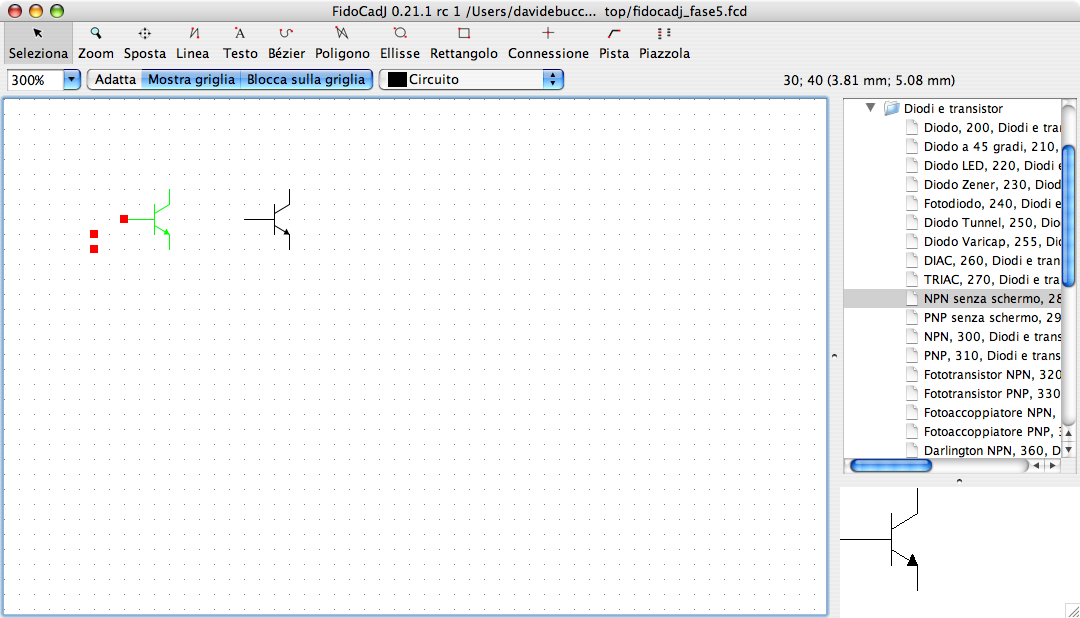
\includegraphics[width=1\textwidth,]{fidocadj_fase1} 

\caption{We start by drawing a couple of transistors.}


\label{fig_fidocadj_fase1} 
\end{figure}


We may notice that the bipolar transistor on the left is not correctly
oriented. To fix the problem is sufficient to click on {}``Select'',
from the toolbar, select the transistor (which will be highlighted
in green, with three control points\index{control point} identified
by small red squares) and then press \keyevidence{S} to obtain
its mirrored version. You may also press \keyevidence{S} when you have selected the symbol in the libraries and you are about to position it in the drawing. We will thus obtain a result similar to the
one shown in figure~\ref{fig_fidocadj_fase2}.

%
\begin{figure}
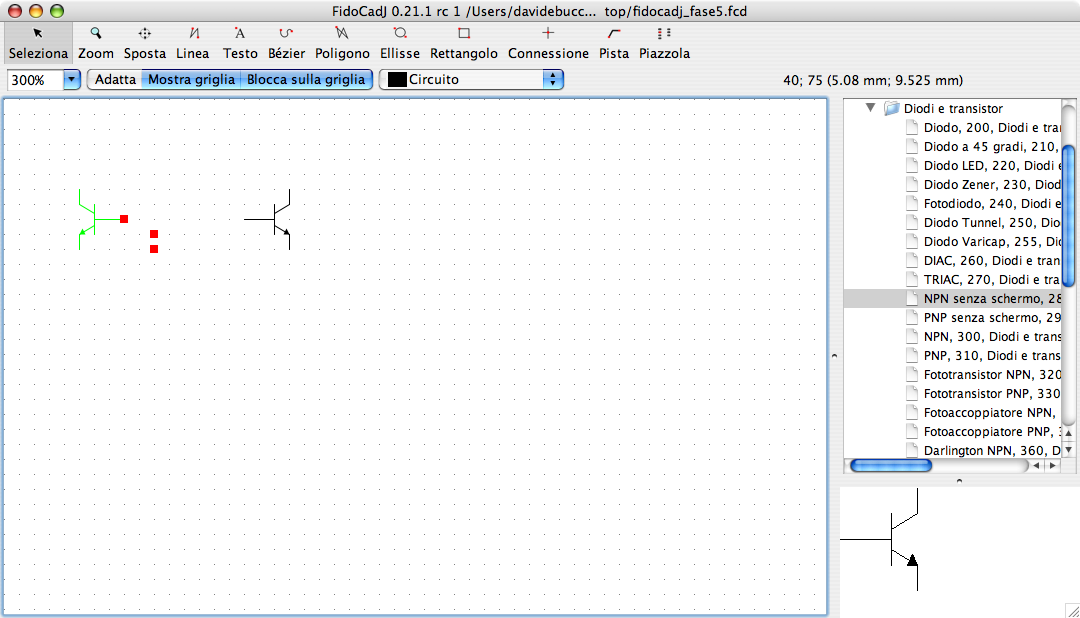
\includegraphics[width=1\textwidth,]{fidocadj_fase2} 

\caption{Select and mirror with \keyevidence{S} the transistor on the left.}


\label{fig_fidocadj_fase2} 
\end{figure}


By using the tool {}``Line'' from the toolbar\index{toolbar}, we
will be able to make a few electrical connections, until we will realize
that we started our drawing to close to the edges of the drawing area.
The issue can be easily fixed by selecting the whole drawing: in {}``Select''
mode, we can click on the upper left corner of the drawing and, holding
the left button of the mouse pressed, drag the cursor up to the lower
right corner. A rectangle with a green contour will appear to indicate
that we are trying to select all the elements included in it. Since
we want to move everything we have drawn so far, we will have to select
them all first(see figure~\ref{fig_fidocadj_fase3}). Now, still
in select mode, we can click on any selected element to drag the selection
to the desired position.

%
\begin{figure}
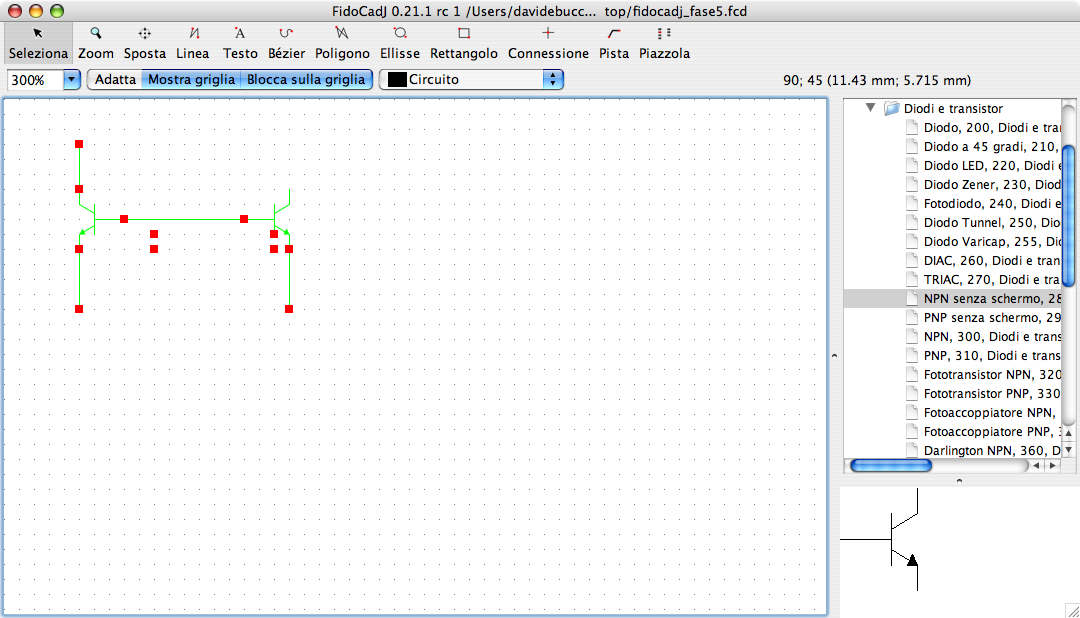
\includegraphics[width=1\textwidth,]{fidocadj_fase3} 

\caption{We are too close to the top edge of the sheet: let's select the whole
drawing and move it toward the centre.}


\label{fig_fidocadj_fase3} 
\end{figure}


We can then continue placing the other parts of the circuit, in particular
a resistor\index{resistor} (Standard Library/Discrete devices/Resistor)
and the label for the positive power supply (Standard Library/Basic symbols/Terminal +). We will need to rotate the latter in order to
place in the desired position. Again, we can select it and press \keyevidence{R}
until we will obtain the desired result. We should now have a screen
similar to the one in figure~\ref{fig_fidocadj_fase4}.

%
\begin{figure}
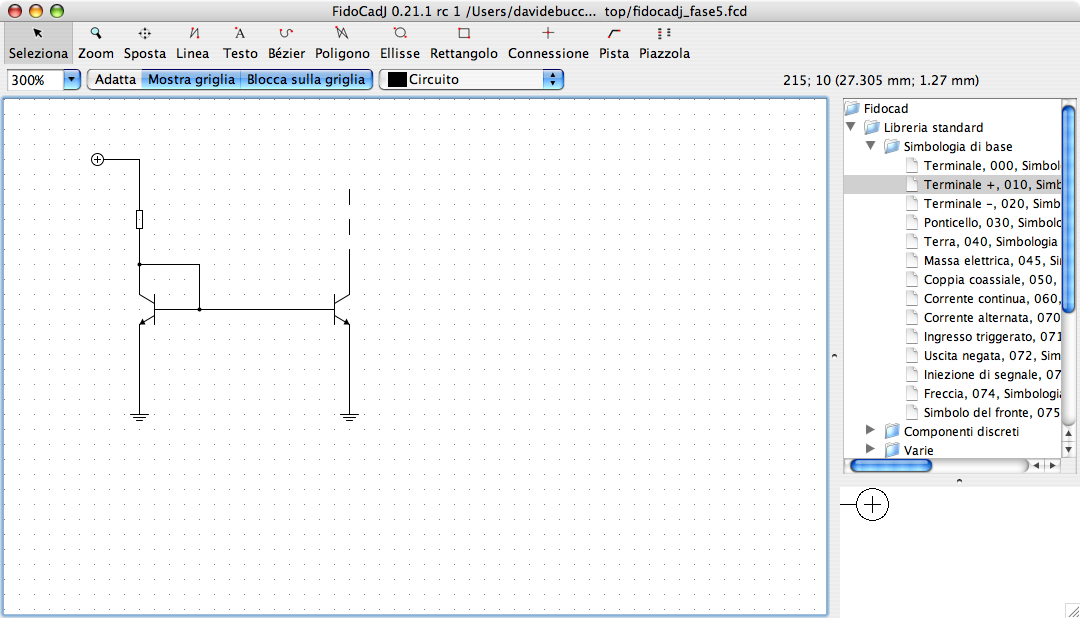
\includegraphics[width=1\textwidth,]{fidocadj_fase4} 

\caption{The circuit almost completed.}


\label{fig_fidocadj_fase4} 
\end{figure}


To complete the schematic we only need to add the text strings and
the arrow to indicate the direction of the current. For the latter
there is a macro called {}``Arrow'', contained in {}``Standard library/Basic symbols''. To place the text, we can press the
button {}``Text''\index{text} from the toolbar e click in the drawing
area on the desired position. As the default text {}``String'' will
be introduced, we will need to modify its characteristics by double-clicking
in select mode (see figure~\ref{fig_param_testo}). The transistor's
part number and name used (it is actually a transistor matched pair
in our example) are specified in the fields {}``Name'' and {}``Value''
which are accessed in select mode by double-clicking on the macro.%
\footnote{The feature which allows us to add a name and a value to a macro or
a component's symbol is actually an extension introduced with FidoCadJ
\index{FidoCadJ extension} not present in the original FidoCad\index{FidoCad}.
See section~\ref{FCJ_extension} for more information on compatibility.%
} The suggested dimension to work with electrical circuits is 4 units
in vertical and 3 units in horizontal. The complete circuit is shown
in figure~\ref{fig_fidocadj_fase5}.

%
\begin{figure}
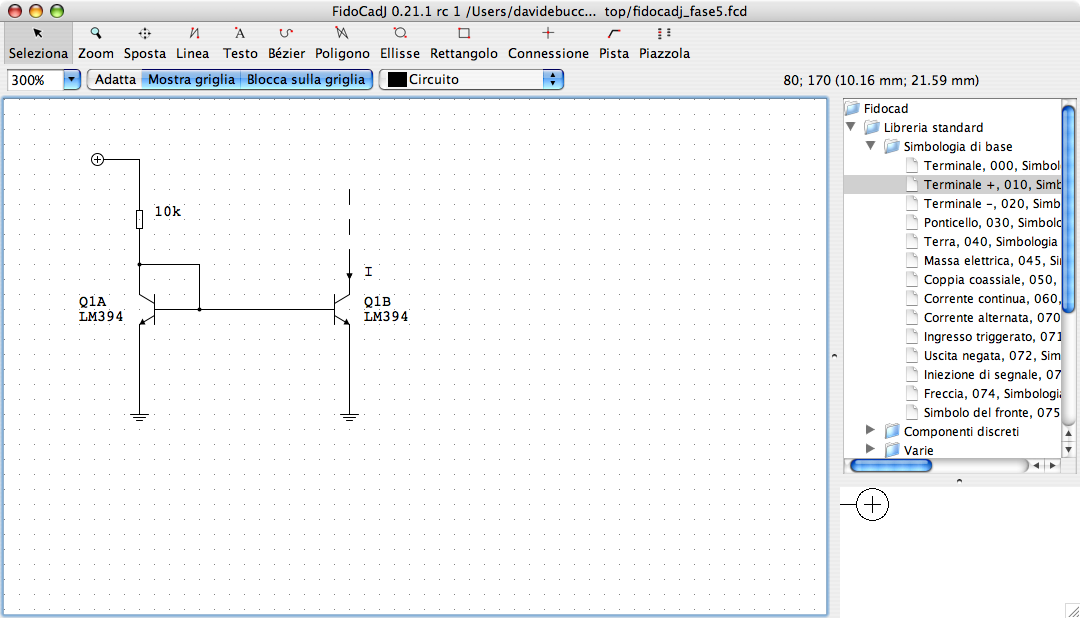
\includegraphics[width=1\textwidth,]{fidocadj_fase5} 

\caption{The final circuit.}


\label{fig_fidocadj_fase5} 
\end{figure}


As a curiosity, this is how the code\index{code} which describes
the circuit of our example looks like. To access this code, it is
sufficient to select {}``Insert Circuit'' from the menu {}``Circuit''.
We are now ready to copy and paste our circuit on an e-mail message
\index{e-mail}, in a newsgroup\index{newsgroup}, or in a forum\index{forum}.
\begin{lstlisting}
[FIDOCAD]
MC 95 65 0 0 280
FCJ
TY 115 60 4 3 0 0 0 * Q1B
TY 115 65 4 3 0 0 0 * LM394
MC 55 65 0 1 280
FCJ
TY 20 60 4 3 0 0 0 * Q1A
TY 20 65 4 3 0 0 0 * LM394
LI 55 65 95 65 0
LI 40 75 40 95 0
LI 110 75 110 95 0
LI 40 40 40 55 0
MC 40 30 0 0 115
LI 40 15 40 30 0
LI 30 15 40 15 0
MC 30 15 2 0 010
LI 40 50 60 50 0
LI 60 50 60 65 0
SA 60 65 0
SA 40 50 0
LI 110 45 110 55 0
LI 110 35 110 40 0
LI 110 25 110 30 0
MC 40 95 0 0 040
MC 110 95 0 0 040
TY 45 30 4 3 0 0 0 * 10 k
TY 115 50 4 3 0 0 0 * I
MC 110 50 1 0 074
\end{lstlisting} 
If you are interested in the export format
used by FidoCad, there is a detailed description on chapter~\ref{chap_formato}.

However, there is no need to use the {}``Insert circuit'' dialog;
we can simply select the entire drawing, copy it (by selecting ``edit/copy''
or by pressing \keyevidence{Ctrl+C} ) and paste it onto the message
we are writing and the code will be added automatically\index{code}.


\section{The layers}

\label{sec_layer} A way to picture a layer\index{layer} is that
of a drawing made on acetate sheets. The final drawing will be given
by the combination of all the layers, which will be superposed like
acetates. Every layer is characterized by a different color and can
be visible or hidden. This approach is common to many CAD\index{CAD}
packages, as it allows an easy representation and management of different
parts of the drawing that will be superposed, as for example in a
PCB design\index{PCB}.

FidoCadJ allows up to 16 layers, numbered from 0 to 15. Conventionally,
some of the layers have a specific purpose. In particular, layer zero
is used for electrical schematics\index{electrical schematic}, layer
1 for the copper soldering side\index{soldering}, layer 2 for the
copper components side and layer 3 for the silk-screen\index{silk-screen}.
The remaining layers do not have any pre-defined purpose and can be
used freely. Name and color\index{colour} of every layer can be
specified using the menu {}``View/Layer''. From the same menu we
can also select the layers that we want to see on screen or that we
want to print.

The layers' ordering is important, as layer with a lower number will
be drawn first. That is, drawings on successive layers may cover the
ones on lower layers.


\section{The grid}

The logic unit\index{logic unit} in FidoCadJ is 5 mils (127 micron)
and ``half units'' are not allowed, meaning that the
coordinates of any graphic element must be integer numbers. This allows
us to obtain a resolution\index{resolution} sufficiently fine to
draw an electrical schematic and the majority of PCBs. However, for
ease of drawing, the application allows us to set a coarser grid and
force the mouse to align with the nearest point of the grid\index{grid}.
To enable this functionality there are two buttons, {}``Show Grid''
and {}``Snap'', which allow toggling between visible/hidden grid
and force the mouse cursor on the grid or let it move freely, respectively.
The grid step can be chosen through a dialog window that can be accessed
from the menu ``File/Options''.


\section{A simple PCB}

To practice what we learnt so far, We will see how to design a simple
PCB. Unlike other software for electronic CAD which are very
powerful but sometimes quite hard to manage, FidoCadJ provides in
practice an electronic version of the good old R41 transfers\index{R41 transfers}.
Obviously, working on a computer allows us to benefit from all the
flexibility offered by the machine.

\marginpar{The reader
will find his way through: a few scribbles made with paper and pencil
(and a lot of erasers) will result in time saved by obtaining a clear
idea to be developed with the use of the computer.} It must be noted that the design of a PCB\index{PCB}, especially
if this is a complex one, is not an easy task.  The autoplacer\index{autoplacer}
and the autorouter\index{autorouter} features promise miracles on
the publicity flyers from major CAD companies. There is no doubt that
these are still a tasks where the user's experience still plays an
important role. FidoCadJ constitutes a very immediate and fast way
to draw small PCBs on a DIY scale. We will see here how to draw a
very simple, yet complete, one.

I would suggest to start with a clear idea of where to place each
component and how to draw all the tracks so that they will cross each
other as less as possible \index{crossing of tracks}.

Here we will cheat a little and we will start from the result we want
to obtain, as shown in figure~\ref{fig_amplificateur}. It is a simple
common-emitter amplifier built around an NPN transistor, type BC547
or similar. It will be useful to think of the board as it was transparent,
by looking from the components side. For this purpose the silk-screen\index{silk-screen}
with the components drawing will be very useful, although probably
we do not want to print it out onto the actual board for a DIY project.

%
\begin{figure}
\centering 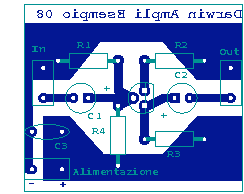
\includegraphics[width=0.5\textwidth]{amplificateur} 

\caption{A very simple amplifier stage using an NPN transistor connected in
a common emitter configuration.}


\label{fig_amplificateur} 
\end{figure}


The first thing I would suggest to do is to place all the components
as best as possible. In our example these would be the transistor
(from the library {}``PCB footprints/3 terminals semiconductors/TO92''),
the resistors ({}``PCB footprints/Resistors/Resistor 1/4 W 0,4 i''),
and the electrolytic capacitors ({}``PCB footprints/Electrolytic capacitor/Vert. diam. 5 mm 2.5 mm pitch''). In order to delimitate
the board, it may be useful to place an empty rectangle on the silk-screen
layer (layer No.~3). To do so we can use the \emph{rectangle} primitive\index{rectangle}
making sure that we selected the appropriate layer first. We should
get a result similar to the one shown in figure~\ref{fig_amplificateur_phase1}.%
\footnote{FidoCadJ is currently available in Italian\index{Italian}, French\index{French}, English\index{English}, Spanish\index{Spanish}, German\index{German} and Chinese\index{Chinese}.
It is quite easy to translate menus and commands, so if you would
like to see FidoCadJ in your native language, please let me know!
There is also work to be done to translate the libraries (at least
the standard ones) and of course this manual.%
}

%
\begin{figure}
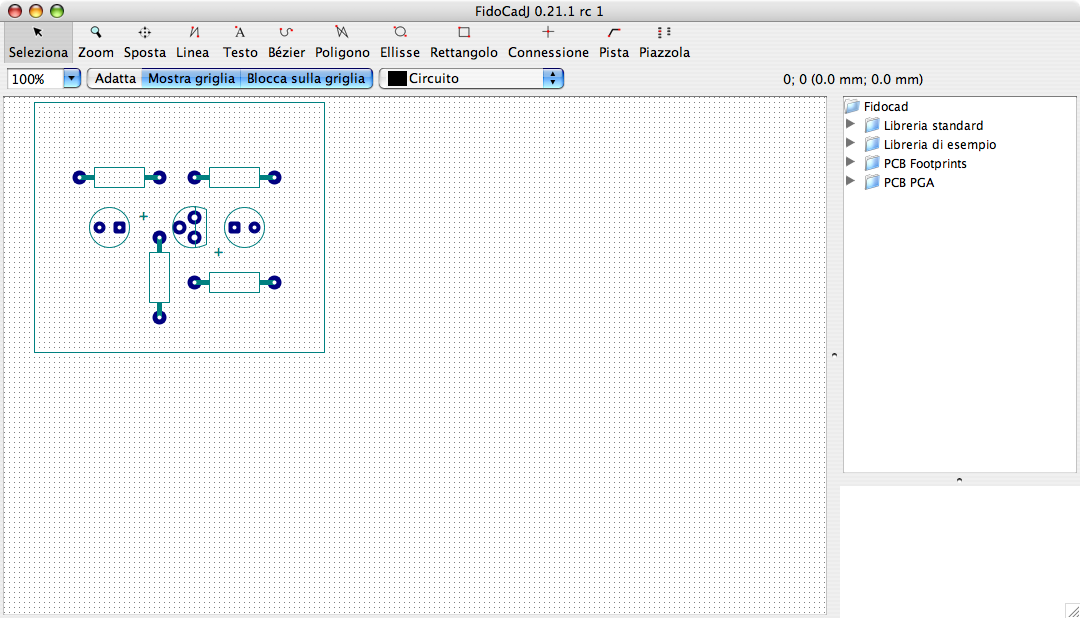
\includegraphics[width=1\textwidth]{amplificateur_phase1} 

\caption{The most important devices are placed on the board.}


\label{fig_amplificateur_phase1} 
\end{figure}


We can then introduce the copper areas which will provide the positive
and negative power supply. These are specified by drawing a polygon\index{polygon}
(using the \emph{poly line} primitive) and double clicking near its border 
in selection mode\index{selection mode} to tell FidoCadJ
(through dialog box) that we want a filled polygon. Before placing
the polygon, make sure that the current layer\index{layer} is the
one where we want to place the copper area (layer No~1, or copper
solder side). The use of a filled area for the power supply lines
may be useful to ensure that these connections will have a low stray
inductance. We should be able to reproduce the result shown in figure~\ref{fig_amplificateur_phase2}.

%
\begin{figure}
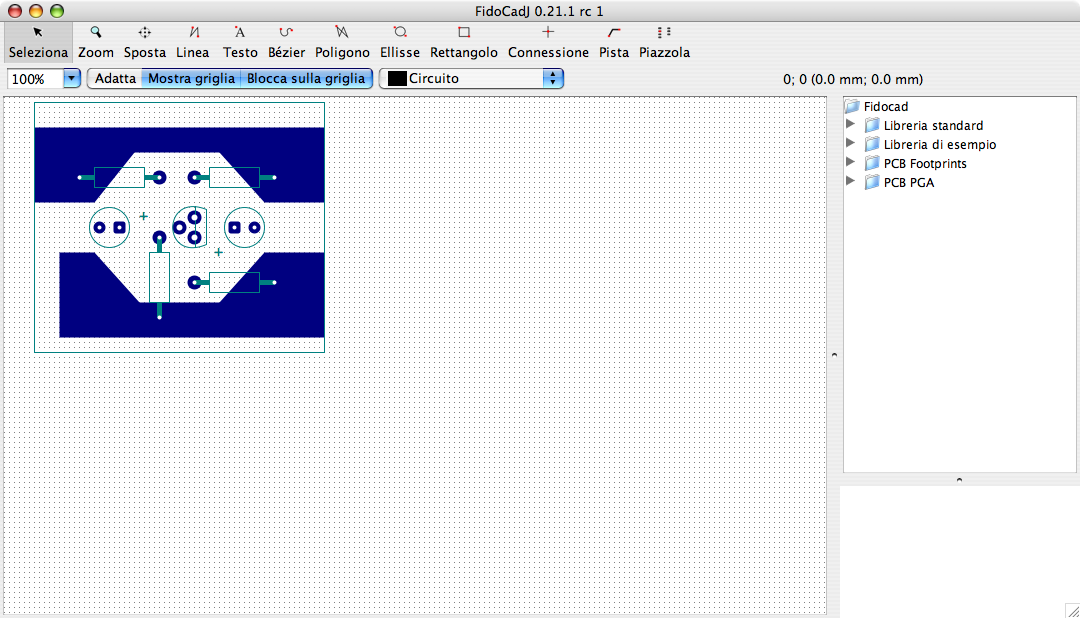
\includegraphics[width=1\textwidth]{amplificateur_phase2} 

\caption{Added the power supply connections using polygonal lines\index{polygon}.}


\label{fig_amplificateur_phase2} 
\end{figure}


To complete the electrical connections we can use the \emph{PCB line}
primitive\index{PCB line}. I chose a track thickness of 10 units
(1.27~mm), which helps the soldering process. %
\begin{figure}
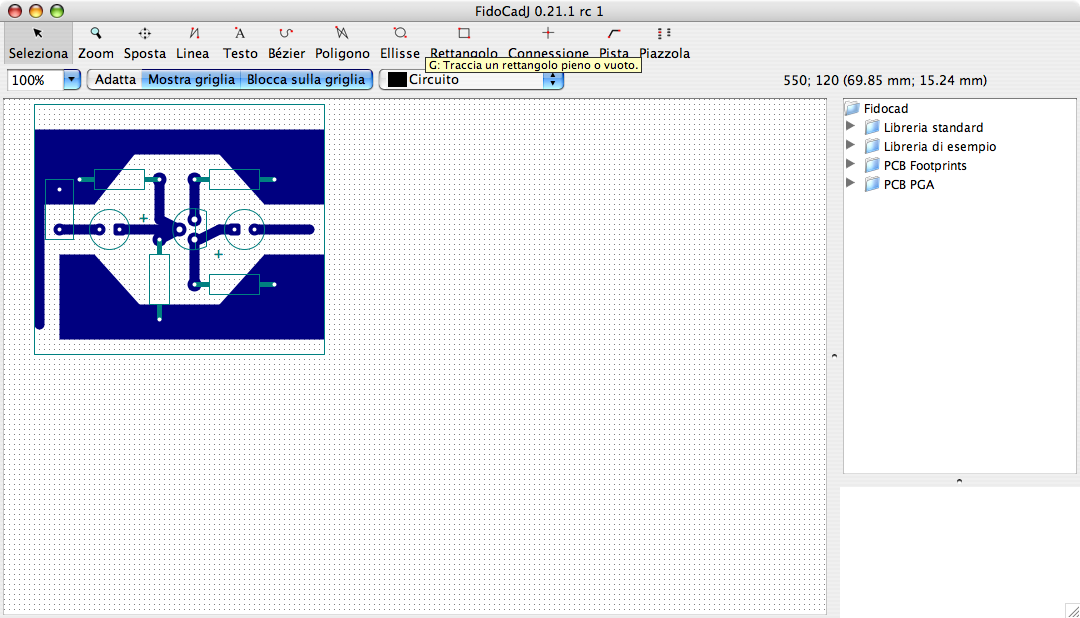
\includegraphics[width=1\textwidth]{amplificateur_phase3} 

\caption{Added the remaining connections PCB tracks\index{PCB track}.}


\label{fig_amplificateur_phase3} 
\end{figure}


We realize that we need a few connectors: one for the input, one for
the output and one for the power supply. We can use the footprint
designed for a polyester capacitor.  It will probably have the right dimensions. Let's
not forget that FidoCadJ is thought as a replacement for the transfers\index{R41 transfers}\dots

We can also place a ``$+$'' and a ``$-$'' on the copper layer and
place a ceramic capacitor in parallel with the power supply. \marginpar{Be careful with the
track widths: something that looks like a motor-way on the screen will
probably be a track so thin that will detach from the board during
the soldering.}
Let us
put the writing on the top side as well. To write on the copper layer,
after selecting the proper layer it will also be necessary to mirror
all the writings\index{writings mirroring}. This is easily done within
the usual properties dialog accessed by double-clicking on the string
we want to modify when we are in selection mode. It will need a few
tries to obtain the right dimensions for the characters. To give an
idea it is useful to have a ratio of 3/4 between the horizontal and
the vertical dimensions of the characters\index{characters dimension}.
Figure~\ref{fig_amplificateur_phase4} shows the result obtained
using 11 units for the horizontal and 18 units for the vertical dimension
of the text.

%
\begin{figure}
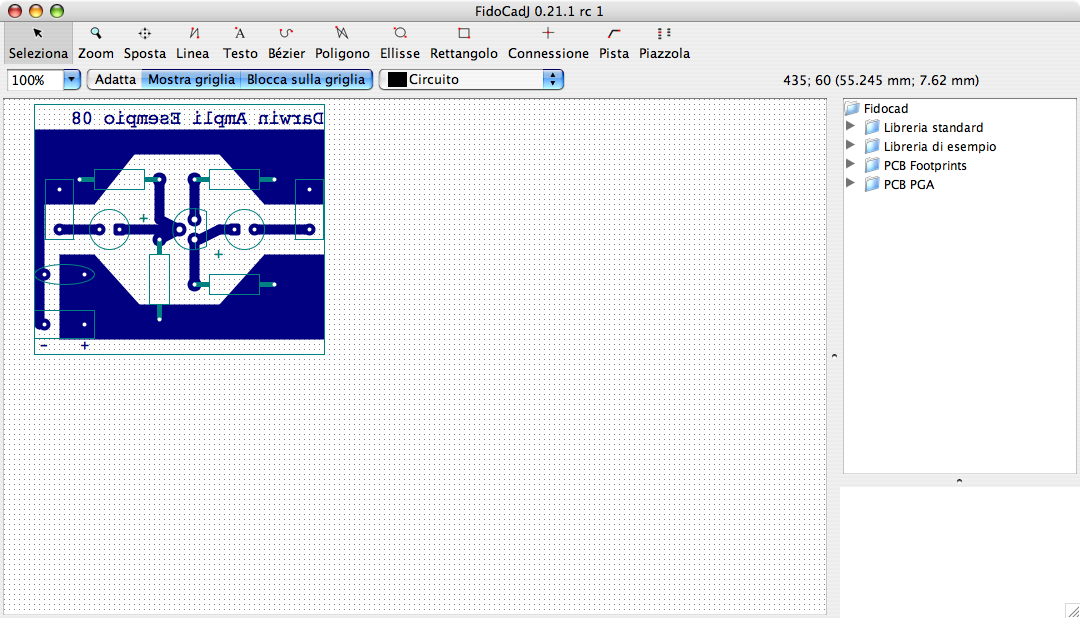
\includegraphics[width=1\textwidth]{amplificateur_phase4} 

\caption{The PCB almost completed\index{PCB}.}


\label{fig_amplificateur_phase4} 
\end{figure}


At this stage the only thing missing is the text with the name of
each component, that can be placed on layer 3 (silk-screen). The program
with the PCB completed is shown in Figure~\ref{fig_amplificateur_complet}.

%
\begin{figure}
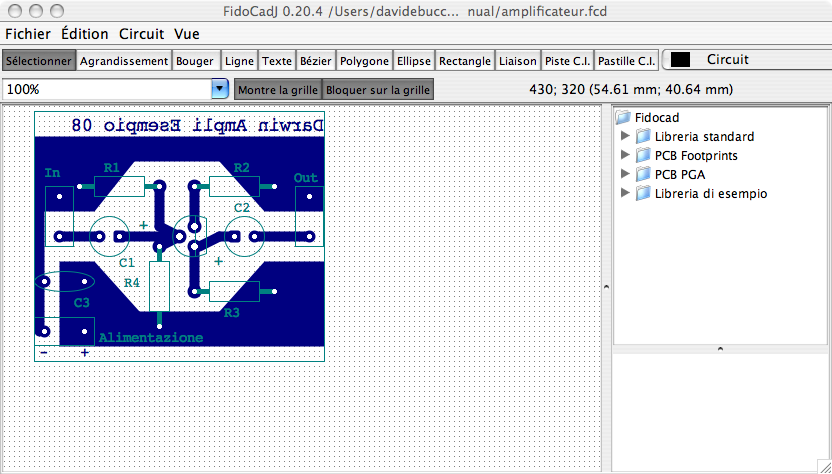
\includegraphics[width=1\textwidth]{amplificateur_complet} 

\caption{The job completed with the silk-screen.}


\label{fig_amplificateur_complet} 
\end{figure}


Once the drawing is completed, we will probably need to print\index{printing}
it either on a transparency to use it with a printing box\index{printing box}
or to use it with other methods such as the ``Press\&Peel''\index{Press&Peel@Press\&Peel}.
To do so we need to make invisible all the layers that we do not want
to print. This is done from the dialog window accessed from the menu
{}``Vista/Layer''. In our case it will be sufficient to hide the
layer 3 containing the silk-screen. The program will show the copper
layer only.

We will then print everything that is shown on the screen (obviously
NOT adapted to the size of the page, as we want to have the dimensions
set in the drawing), taking care of selecting the black and white
printing to ensure the maximum contrast. It may be useful to mirror
the whole drawing, depending on the technique chosen for the production
of the PCB\index{PCB}. Since our PCB is quite small, in its real
dimensions it will occupy only a small corner of the sheet (assuming
a standard ISO-UNI A4\index{A4}), as we can see in Figure~\ref{fig_amplificateur_impression}.

%
\begin{figure}
\centering \fbox{ 
\includegraphics[width=0.6\textwidth]{amplificateur_impression}} 

\caption{The PCB, as it appears when printed (mirrored) on a ISO-UNI A4 sheet.}


\label{fig_amplificateur_impression} 
\end{figure}


For information, below is the code generated for the PCB of the example
above (be careful with long lines!):
\begin{lstlisting}
[FIDOCAD]
TY 320 10 18 11 0 4 1 * Darwin Ampli Esempio 08 
TY 85 240 12 8 0 5 1 * + 
TY 44 239 12 8 0 5 1 * - 
PL 35 90 35 225 10 1
PL 55 130 95 130 10 1
PL 250 130 305 130 10 1
PL 215 130 230 130 10 1
PL 195 140 215 130 10 1
PL 115 130 175 130 10 1
MC 155 220 3 0 PCB.R01
MC 75 80 0 0 PCB.R01
MC 270 185 2 0 PCB.R01
MC 270 80 2 0 PCB.R01
MC 230 130 3 0 PCB.CE00
MC 115 130 1 0 PCB.CE00
MC 40 175 0 0 PCB.CC50
PL 190 80 190 120 10 1
PL 190 140 190 185 10 1
PL 155 80 155 120 10 1
PL 155 120 175 130 10 1
PL 155 140 175 130 10 1
PP 30 30 30 105 90 105 130 55 215 55 260 105 320 105 320 30 1
PP 320 240 320 155 260 155 215 205 135 205 90 155 55 155 55 240 1
MC 190 120 0 0 PCB.TO92
MC 305 90 1 0 PCB.CPBX352
MC 55 90 1 0 PCB.CPBX352
MC 80 225 2 0 PCB.CPBX352
TY 290 65 12 8 0 0 3 * Out 
TY 40 60 12 8 0 0 3 * In 
TY 95 225 12 8 0 0 3 * Alimentazione 
TY 70 190 12 8 0 0 3 * C3 
TY 230 95 12 8 0 0 3 * C2 
TY 115 150 12 8 0 0 3 * C1 
TY 120 170 12 8 0 0 3 * R4 
TY 220 200 12 8 0 0 3 * R3 
TY 230 55 12 8 0 0 3 * R2 
TY 100 55 12 8 0 0 3 * R1 
RV 30 5 320 255 3
\end{lstlisting} 

\section{Using the ruler}\index{ruler}
When drawing a PCB, it is often useful to measure distances in the working area. For example, you can check a track width, the clearance between two tracks or the total size of a card. FidoCadJ offers (from version 0.23.2) a ruler feature which allows you to easily perform those tasks. Just right click and drag. You should obtain a green ruler, like the one shown in figure~\ref{fig_fidocadj_righello}. If the right click and drag action is not used in your operating system, you can alternatively left click and drag while pressing the \keyevidence{Shift} key.
\begin{figure}
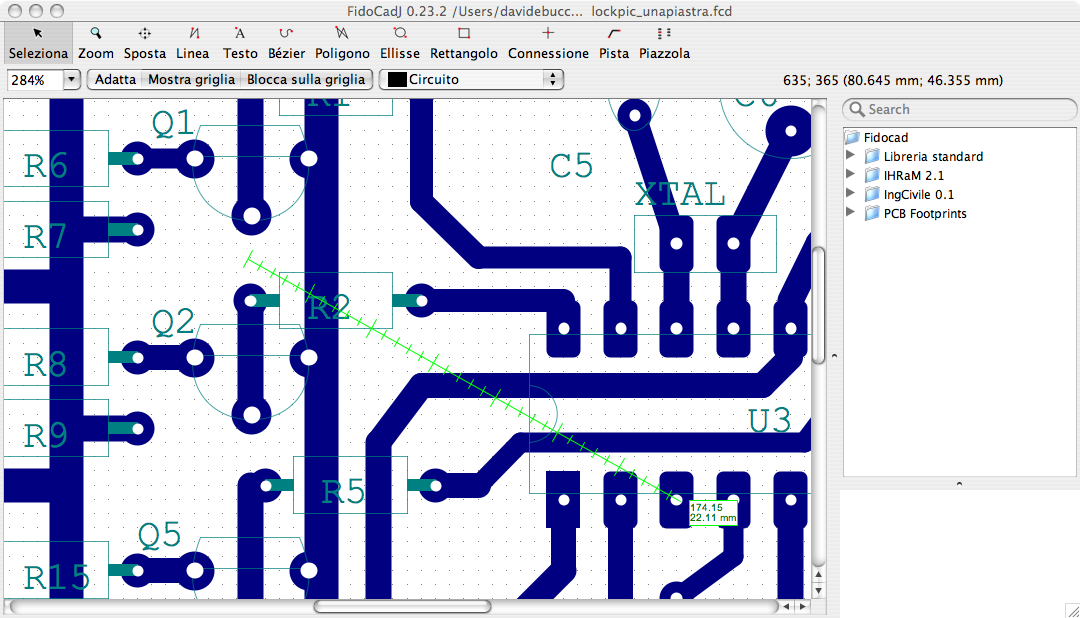
\includegraphics[width=\textwidth]{fidocadj_righello}
\caption{Right click and drag to activate the FidoCadJ ruler.}
\label{fig_fidocadj_righello}
\end{figure}
The total length measured is shown in FidoCadJ logical units\index{logical unit} as well as in millimeter. This is useful when the drawing is printed in the 1:1 mode (such as for PCB's).

\section{Arrow and stroke styles}
FidoCadJ allows to draw arrow heads\index{arrows} at the beginning and at the end of lines, B�zier curves and natural cubic splines. It also allows you to specify whether the arrow should be at the beginning or at the end of an element (or both), and offers you a few different arrow styles.

A few stroke styles\index{stroke styles} are now available for technical or mechanical drawings. Figure~\ref{fig_gyrator} shows an example in which an electrical circuit (a GIC\index{GIG}) is enclosed in a dashed rectangle. An arrow at the end of a B�zier curve is also being used. By doing double-click on this element, FidoCadJ shows a parameter window which should be similar to the one shown in figure~\ref{fig_parametri_bezier}. You can notice that the option box ``Arrow at start'' has been checked. FidoCadJ will thus trace an arrowhead by taking care of his orientation.
There are several different drawing styles for the arrow\index{arrow styles} as well for dashing \index{dashing styles}. You may try to play a little bit with them to appreciate their differences.

\begin{figure}
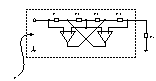
\includegraphics[width=\textwidth]{gyrator}
\caption{An electrical drawing (an Antoniou's GIC) in which some FidoCadJ extensions have been used.}
\label{fig_gyrator}
\end{figure}
\begin{figure}
\centering
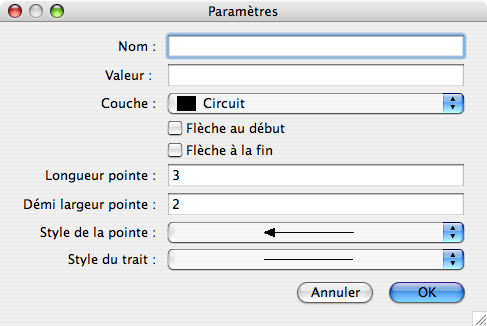
\includegraphics[width=.7\textwidth]{parametri_bezier}
\caption{The parameter window of the B�zier curve shown used in the schematics of figure~\ref{fig_gyrator}}
\label{fig_parametri_bezier}
\end{figure}
The possibility of choosing a dashing style and putting arrowheads was not comprised in the original FidoCad format. This unfortunately means that FidoCadJ drawings using those functionalities are not completely backward compatible with FidoCad\index{FidoCad} per Windows.
When you do chose to use a FidoCadJ extension, you need to know what you are doing. If you need to have a complete FidoCad compatibility, you can activate the option ``Strict FidoCad compatibility'' in the ``FidoCadJ extensions'' tab of the ``FidoCadJ preferences'' window. In this way, the program will not allow you to introduce graphical elements which would give compatibility problems with FidoCad. If you need more details about the compatibility of the new graphical elements with FidoCad\index{FidoCad}, have a look at section~\ref{FCJ_extension}.


\section{Exporting}

One of the most important thing to me about FidoCadJ is the possibility
to create simple schematics for typographic use. For this reason I
introduced a feature that allows the exportation\index{exportation}
of drawings through a number of different file formats. 

To export the current drawing, select the command {}``Export'' from
the menu {}``File''. The Table~\ref{tab_esportazione} shows a
list of graphic file formats currently available. \marginpar{A vectorial
format\index{vectorial format} stores the elements that compose
the drawing. A bitmap format\index{bitmap format} works on a matrix
of pixels.} For every file format, the Table (but also the export dialog
in FidoCadJ) specifies whether it is vectorial or bitmap. Whenever
possible it is better to choose a vectorial format to obtain the best
results.%
\footnote{The code structure of FidoCadJ allows the addition of other file format
quite easily. Please contact me if you like to participate to the
project.%
}

For the bitmap file formats it may be useful to enable the option
{}``Anti aliasing'', to reduce the annoying effect of the quantization,
visible especially on diagonal lines. The resolution and the {}``Anti
aliasing'' options are not used when exporting to a vectorial file
format. In this case, you may instead specify a scaling factor.

The option {}``Black\&White'' allows the printing of any visible
layer in solid black. This is important for the preparation of films
to be used for typographic purposes or with a printing box. %
\begin{table}
\centering \begin{tabular}{lp{0.7\textwidth}}
\toprule Format  & Comment\tabularnewline
\midrule \textsc{jpg}\index{JPG}  & Very diffused bitmap format. Since the compression used is lossy\index{lossy compression},
it is not suitable to for exporting FidoCadJ schematics. It is made
available due to its diffusion. \tabularnewline
\textsc{png}\index{PNG}  & Compressed bitmap format, suitable for exporting schematics. This
is probably the best way to export a FidoCadJ drawing when a vectorial
format cannot be used. \tabularnewline
\textsc{svg}\index{SVG}  & W3C standard vectorial format. Some internet browsers (such as the
recent versions of Safari\index{Safari}) allow its visualization
within a web page. Very good format for graphics and schematics, it
enables the use in applications such as Inkscape\index{Inkscape}
to modify the drawings made with FidoCadJ. There are currently some
limitations with the exportation of rotated and mirrored text. \tabularnewline
\textsc{eps}\index{EPS}  & Encapsulated Postscript vectorial format\index{Postscript}. Very
useful to those who use professional graphics applications, or want
to use a FidoCadJ drawing in a \LaTeX{}\index{\LaTeX{}@\LaTeX} document.
The drawings exportation should be fully working. This is the option
used to obtain Figure~\ref{fig_amplificateur}, page~\pageref{fig_amplificateur}
in this manual (passing through a \textsc{pdf} conversion, since I
use \textsc{pdf}\LaTeX{}\index{pdf\LaTeX{}@\textsc{pdf}\LaTeX}). \tabularnewline
\textsc{pgf}\index{PGF}  & Vectorial format to be used directly in a \LaTeX{}\index{\LaTeX{}@\LaTeX}
document, when using the \textsl{pgf} package, available in the CTAN
archive. This exportation option was thought in particular to export
schematics and uses an easily editable script. The text attributes
will not be translated. This allows the introduction of \LaTeX{}\index{\LaTeX{}@\LaTeX}
code directly into the drawing and it is the technique used in this
manual to obtain Figure~\ref{fig_schema}, page~\pageref{fig_schema}. \tabularnewline
\textsc{scr}\index{SCR}  & FidoCadJ allows the exportation of a drawing
to a script that can be imported in CadSoft\index{CadSoft} Eagle\index{Eagle}.
To use this feature, it is necessary to install the library \lstinline!FidoCadJLIB.lbr!
into the directory \lstinline!lbr! of the current installation of
Eagle. The library can be downloaded from FidoCadJ's website. At the
time of writing, this option works only with schematics containing
only the most common symbols. Some drawing elements such as pads and
tracks are not available yet. These will not be exported to the Eagle
script.\tabularnewline
\bottomrule  & \tabularnewline
\end{tabular}

\caption{List of all the export file formats available in FidoCadJ.}


\label{tab_esportazione} 
\end{table}



\section{Command line options}

The application is distributed as a file \lstinline!.jar!\index{jar},
which is a Java archive.%
\footnote{Except for the Macintosh\index{Macintosh} version, which is a stand
alone application.%
} In many operating systems, to run the application it should be enough
to double-click on the file, provided that a recent version of Java\index{Java}
is installed on the machine. Using Sun's\index{Sun} terminology,
the so called JRE\index{JRE}, or the Java Runtime Environment, is
all that is needed to run a program written in Java (but not to write
it: in that case the SDK would be necessary\dots). The minimum Java
version needed to run FidoCadJ is the 1.5, which has been around for
a few years now.

In some cases, it may be useful to run FidoCadJ from a command line
(the terminal\index{terminal} in the Unix\index{Unix} systems, or
the MS-DOS\index{MS-DOS prompt} Prompt in Windows\index{Windows}).
To do so, it is sufficient to run the command \lstinline!java!, with
the option \lstinline!-jar!: 
\begin{lstlisting} 
java -jar fidocadj.jar
\end{lstlisting}

If a file is specified in the command line\index{command line}, FidoCadJ
will try to open it. For example (on a Unix\index{Unix} machine):
\begin{lstlisting} 
java -jar fidocadj.jar ~/FidoCadJ/test.fcd 
\end{lstlisting}

FidoCadJ will be run and it will try to open the file \lstinline!~/FidoCadJ/test.fcd!
(provided that this exists).

There are some other interesting things FidoCadJ can do.
Option \lstinline!-h! shows a listing of the FidoCadJ options:
\lstset{basicstyle=\scriptsize\ttfamily}
	 	 
\begin{lstlisting}
[davidebucci@Darwin]$ java -jar fidocadj.jar -h

This is FidoCadJ, version 0.24.1.
By Davide Bucci, 2007-2012.

Use: java -jar fidocadj.jar [-options] [file] 
where options include:

 -n     Do not start the graphical user interface (headless mode)

 -d     Set the extern library directory
        Usage: -d dir
        where 'dir' is the path of the directory you want to use.

 -c     Convert the given file to a graphical format.
        Usage: -c sx sy eps|pdf|svg|png|jpg|fcd|sch outfile
        If you use this command line option, you *must* specify a FidoCadJ
        file to convert.
        An alternative is to specify the resolution in pixels per logical unit
        by preceding it by the letter 'r' (without spaces), instead of giving
        sx and sy.

 -s     Print the size  of the specified file in logical coordinates.

 -h     Print this help and exit.

 -t     Print the time used by FidoCadJ for the specified operation.

 -p     Do not activate some platform-dependent optimizations. You might try
        this option if FidoCadJ hangs or is painfully slow.

 -l     Force FidoCadJ to use a certain locale (the code might follow
        immediately or be separated by an optional space).

 [file] The optional (except if you use the -d or -s options) FidoCadJ file to
        load at startup time.

Example: load and convert a FidoCadJ drawing to a 800x600 pixel png file
        without using the GUI.
  java -jar fidocadj.jar -n -c 800 600 png out1.png test1.fcd

Example: load and convert a FidoCadJ drawing to a png file without using the
        graphic user interface (the so called headless mode).
        Each FidoCadJ logical unit will be converted in 2 pixels on the image.
  java -jar fidocadj.jar -n -c r2 png out2.png test2.fcd

Example: load FidoCadJ forcing the locale to simplified chinese (zh).
  java -jar fidocadj.jar -l zh


[davidebucci@Darwin]$
\end{lstlisting}
\lstset{language=FIDOCAD,
    basicstyle=\small\ttfamily}
    
The most simple option is \lstinline!-n!, with which the software\dots\ does nothing, i.e. it does not activate the GUI and just exits. In this case, the Java environment variable \lstinline!java.awt.headless! is set to true.
Obviously, this option is not so much useful alone, but it will be precious when using in combination with other functionalities we are about to describe.
Option \lstinline!-d! allows to specify the directory where FidoCadJ will seek for libraries to be loaded at startup. Option \lstinline!-c! allows to make FidoCadJ convert a FidoCad file (which must be specified) into an image in a vector or raster format. This can be very useful, as FidoCadJ can be used as a converter in a non interactive way (along with the \lstinline!-n! option)

We can thus have a look at the first example given in the help:
	 	
\begin{lstlisting}
java -jar fidocadj.jar -n -c 800 600 png out1.png test1.fcd
\end{lstlisting}

FidoCadJ will run without activating the GUI and will export in the png\index{PNG} format the file \lstinline!test1.fcd!. The output file will be called \lstinline!out1.png! and will have a 800x600 pixel size.
There is an alternative version of the  \lstinline!-c! option, which will allow to specify how many pixels should be used to convert one logical unit (we will call this factor $r_\mathrm{p}$). FidoCadJ does not deal with half logical units (they are always integers), by choosing, let's say, $r_\mathrm{p}$ equal to two pixels per logical unit ensures that schematics will be always understandable (even if probably a little bit small). The $r_\mathrm{p}$ factor can be non integer, as in the following example:

\begin{lstlisting}
java -jar fidocadj.jar -n -c r1.25 png out2.png test2.fcd
\end{lstlisting}

To know the total size (in logical units) of a schematic, you can use the \lstinline!-s! option. Remember anyway that, during the exports, FidoCadJ adds always a $t_\mathrm{margin}=3$ logical units margin for each side of the drawing. So, if $t_\mathrm{w}$ is the width of the drawing in logical units given by \lstinline!-s!, you might expect that $p_\mathrm{w}$ the width of your drawing in pixel is calculated as follows:

\begin{equation}
p_\mathrm{w} = r_\mathrm{p} (t_\mathrm{w}+ 2 t_\mathrm{margin})
\end{equation}

Another interesting option, although a feature due to Java\index{Java}
more than FidoCadJ, is the possibility to modify the look of the application
(in the jargon of Java called look \& feel\index{look  feel@look \& feel}).
You can choose the look\&feel that you like without modifying a single
line of code. Here is something that Linux\index{Linux} users appreciate,
the GTK+\index{GTK+} look: 
\begin{lstlisting} 
java -Dswing.defaultlaf=com.sun.java.swing.plaf.gtk.GTKLookAndFeel -jar fidocadj.jar 
\end{lstlisting} 
There is also the classic Motif\index{Motif}
look \& feel, shown in Figure~\ref{fig_fidocadj_motif}\footnote{This style may somehow shock those well acquainted with very refined graphical interfaces such as Aqua, with MacOSX. However, I saw a few years ago a synchrotron control system which had a graphical interface based on Motif. Pretty though stuff!}: 
\begin{lstlisting}
java -Dswing.defaultlaf=com.sun.java.swing.plaf.motif.MotifLookAndFeel -jar fidocadj.jar 
\end{lstlisting} %
\begin{figure}
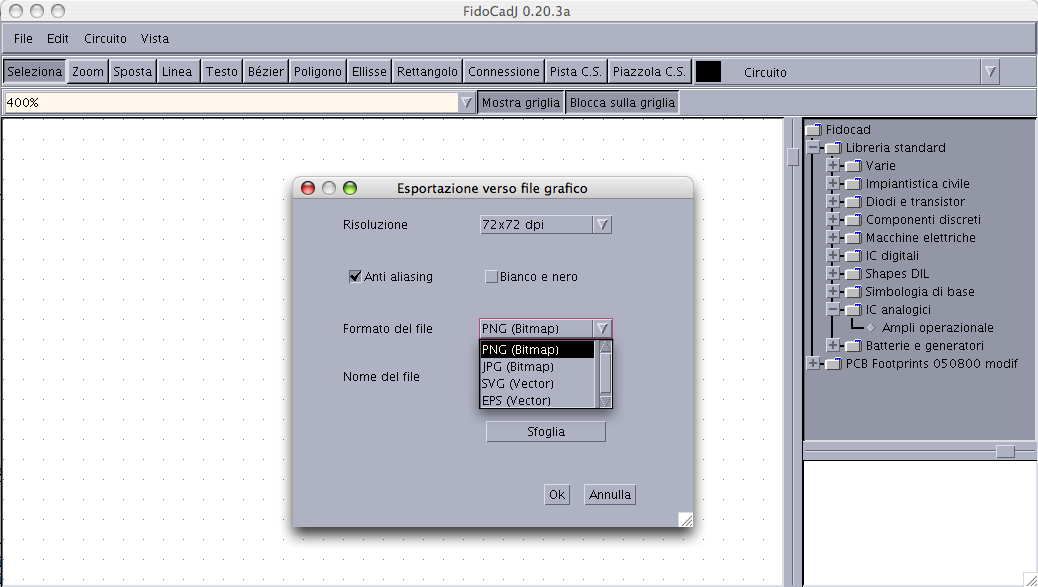
\includegraphics[width=1\textwidth]{fidocadj_motif} 

\caption{The appearance of the program on MacOSX\index{MacOSX}, using the Motif look \& feel.}

\label{fig_fidocadj_motif} 
\end{figure}


Obviously, the commands listed above are meant to be sent from a terminal,
making sure that the current directory contains the file \lstinline!fidocad.jar!
and writing everything on the same line.

\lstset{language=FIDOCAD,
 basicstyle=\small\ttfamily}

\section{Libraries management}

The program allows us to specify a directory in which all the library\index{library} files are placed (extension \lstinline!.fcl!). This can be done through the menu {}``File/Options''. If a file named \lstinline!FCDstdlib.fcl!
is present, its content will supersede the standard library\index{library!standard library} directly available in the application. Analogously, if a file named
\lstinline!PCB.fcl! is present, its content will replace the PCB
library\footnote{Pay attention to the use of capital letters, in particular if your
operating system distinguish uppercase and lowercase letters in the
files management.}.
Other files with \lstinline!.fcl! extension are considered as add-on
libraries and loaded together with the standard library. 
From version 0.23, thanks to Roby IZ1CYN, I could include the IHRaM 3.1 library\index{IHRaM library} directly inside the FidoCadJ distribution. I have done this because among all the libraries I have seen, this one has appeared to be one of the most complete and rationally constructed.
Exactly as it happens for the other libraries embedded in FidoCadJ, if there is a file called \lstinline!IHRAM.FCL! in the current library search path, this one will be loaded at the place
of the version embedded in the program. You also have an electrical symbols library whose file is called \lstinline!elettrotecnica.fcl!.


Other files with \lstinline!.fcl! extension in the library search path will be considered as libraries and FidoCadJ will try to load them when it is starting. This is done when the application starts, when the user change the library search path, or when the ``Update libraries'' option in the ``Circuit menu'' is chosen.

From version 0.23, FidoCadJ allows to split non standard macros (as the original FidoCad\index{FidoCad} does). This can be very useful when posting a drawing in a newsgroup, since in this way each macro which does not belong to the standard FidoCad\index{FidoCad} libraries is expanded into its graphic primitives. The reader thus does not need to have the very same libraries you have installed in your system to read your post.
To activate this behaviour, you have to activate ``Split non standard macros'' in the ``FidoCadJ extensions'' tab of the ``Preferences'' window. You can choose if you want to do that when saving files or when doing a copy/paste of parts of the drawing.

\chapter{Drawing format, macros and FidoCad libraries} \label{chap_formato}

This chapter contains a detailed description of the format used by
FidoCad and, as a consequence, by FidoCadJ to store a drawing. It
is a simple text format which has the advantage of being very compact
and efficient. Since the format has never been described in detail
in a document, I will try to summarize all that I learnt about it.
Since I added a few extensions which are only available on FidoCadJ, I will try to describe them here as well. Remember that from version 0.23.4, FidoCadJ uses only the UTF-8\index{UTF-8} encoding\index{encoding} on all platforms.

\section{Header description}

All the files containing a drawing in the FidoCad \emph{\index{FidoCad}}
format must start with the tag \emph{\lstinline!{[}FIDOCAD{]}!.}
A program can therefore recognize the presence of FidoCad commands
by reading this tag. In this regard, FidoCadJ is more tolerant
than the original FidoCad \emph{\index{FidoCad}} and it recognizes
and correctly interprets a file that does not contain the standard
header\emph{\index{header}}. Even commands containing text can therefore
be interpreted correctly as long as the number of incorrect
lines does not exceed a value set internally in the program (approx.
100). This ensures that FidoCadJ does not waste time working for a
few minutes for example trying to open a very large binary file.


\section{Coordinates system}

FidoCadJ works on a very simple coordinates system\emph{\index{coordinates system}}.
In practice, it has at its disposal a very large area identified only
by whole and positive coordinates. The length of every unit in x and
in y is fixed at \emph{$127\micron$}, a value that allows us to obtain
a good resolution for even the smallest SMD package without being
too fine for everyday use. In typographical terms, the FidoCadJ resolution is 200 dots per inch.

The original FidoCad\emph{\index{FidoCad}} had two different modes
of operation: PCB\emph{\index{PCB}} and electrical
schematic\index{electrical schematic}. In FidoCadJ this difference
has been blurred and appears only at the moment of printing the drawing.
It would therefore be advisable to set the program to resize an electrical
schematic to make better use of the size of the page, otherwise the printed result will have the size of a postage stamp.

\section{Drawing elements}

\label{sec_primitive} FidoCadJ can manage 12 drawing elements as
follows
\begin{itemize}
\item Line\index{line}
\item Filled or empty rectangle\index{rectangle} 
\item Simple text (obsolete)
\item Advanced text\index{text}
\item Filled or empty polyline\index{polyline}
\item Filled or empty ellipse\index{ellipse} 
\item B�zier curve \index{B�zier} 
\item Natural cubic spline curve \index{spline}
\item Electrical junction\index{connection}
\item PCB pad\index{PCB pad}
\item PCB track\index{PCB track}
\item Macro\index{macro}
\end{itemize}
We will proceed by analyzing each of them. In general, every element\index{element}
is identified by a command and a number of parameters\index{parameters}
(usually integer numbers or text strings) placed on the same line
and separated by a space character.


\subsubsection{Line}

The line primitive\index{line}\marginpar{Mathematicians would probably
find the term ``segment''\index{segment} more appropriate.} is identified
by the command \lstinline!LI!\index{LI} and its definition requires
only the begin and end coordinates and the layer: 
\begin{lstlisting}
LI x1 y1 x2 y2 l 
\end{lstlisting} 
the points $(x_{1},y_{1})$ and
$(x_{2},y_{2})$ represent respectively the initial and final coordinates,
while $l$ is the layer, characterized by an integer number between 0
and 15.

\textbf{FidoCadJ extension}: starting from FidoCadJ version 0.23, \lstinline!LI!\index{LI} can be followed in the next line by an extension:
\begin{lstlisting} 
FCJ a b c d e nv
\end{lstlisting}
where $a$ is an integer which represent the presence or not of the arrow heads at the extremes of the segment (have a look at table~\ref{tab_frecce_estremita}), $b$ represents the arrow head style (as table~\ref{tab_frecce_stile}). Parameters $c$ and $d$ give respectively the total length and the half width of the arrow head, while $e$ is an integer which gives the dash style. If $nv$ is equal to 1, the \lstinline!FCJ! command should be followed by two \lstinline!TY! commands giving the name and the value associated to this element.

\begin{table}
\centering

\begin{tabular}{ccp{.7\textwidth}}
\toprule
$a$	& Arrow head \\
\midrule
0	& none \\
1	& at the start side\\
2	& at the end side\\
3	& both sides\\
\bottomrule
\end{tabular}
\caption{Meaning of the $a$ parameter for the presence of an arrow head at the sides of a line or B�zier primitive.}
\label{tab_frecce_estremita}
\end{table}

\begin{table}
\centering
\begin{tabular}{ccp{.7\textwidth}}
\toprule
$b$	& Arrow head style \\
\midrule
0	& filled standard arrow head \\
1	& filled standard arrow head with quota line \\
2	& empty arrow head\\
3	& empty arrow head with quota line\\
\bottomrule
\end{tabular}
\caption{Meaning of the $b$ parameter for the arrow head style.}
\label{tab_frecce_stile}
\end{table}

\subsubsection{Filled or empty rectangle}

A rectangle\index{rectangle} filled or empty is identified by the
commands \lstinline!RP!\index{RP} and \lstinline!RV!\index{RV}
respectively, followed by the coordinates of the two vertices on one
of the two diagonals, and the layer. 
\begin{lstlisting} 
RP x1 y1 x2 y2 l 
RV x1 y1 x2 y2 l 
\end{lstlisting} the points $(x_{1},y_{1})$
and $(x_{2},y_{2})$ represent the two vertices and $l$ is the layer,
characterized by a whole number between 0 and 15.

\textbf{FidoCadJ extension}: starting from FidoCadJ version 0.23,  \lstinline!RP!\index{RP} and \lstinline!RV!\index{RV} can be followed in the next line by an extension:
\begin{lstlisting} 
FCJ e nv
\end{lstlisting}
where $e$ is an integer giving the dashing style. If $nv$ is equal to 1, the \lstinline!FCJ! command should be followed by two \lstinline!TY! commands giving the name and the value associated to this element.


\subsubsection{Simple text (obsolete)}

The simple text \index{simple text} was the first primitive provided
with the early versions of FidoCad\index{FidoCad}. FidoCadJ recognizes
it and simply writes text with size 12, regardless the current zoom\index{zoom}.

Since this primitive was considered obsolete\index{obsolete} by Lorenzo
Lutti\index{Lorenzo Lutti}, the creator of FidoCad\index{FidoCad},
FidoCadJ does exactly the same and, although this is correctly interpreted,
it is not available on the toolbar. FidoCadJ will store this element
exactly as it was advanced text and it will use the command \lstinline!TY!\index{TY}
when saving the file.

The command is \lstinline!TE!\index{TE} and the format is as follows:
\begin{lstlisting} 
TE x1 y1 �text to be written 
\end{lstlisting}
the point $(x_{1},y_{1})$ is where the string {}``text to be written''
will be positioned. Notice that the layer information is missing.
FidoCadJ will treat this object as it was placed on layer zero (circuit\index{circuit}).


\subsubsection{Advanced Text}

The primitive advanced text\index{advanced text} offers much more
flexibility with respect to simple text\index{simple text} introduced
above.

It is identified by the command \lstinline!TY!\index{TY}, followed
by a number of parameters to determine the text orientation (rotated\index{text!rotated}
or mirrored\index{text!mirrored}), as well as dimensions along $x$
and $y$ and the font used. Due to the quantity of information to
provide, the resulting command string is quite complex: 
\begin{lstlisting}
TY x1 y1 sy sx a s l f �text to be written 
\end{lstlisting}
The point $(x_{1},y_{1})$ is where the string ``text to be written''
will be positioned. The value of $s_{y}$ and $s_{x}$ indicates the
horizontal and vertical dimensions of the text in logical units\index{logical unit}.
I chose to let FidoCadJ respect the vertical dimension starting from
the horizontal one, and that aspect ratio will be chanced only if
this is strictly necessary. The text rotation is managed by the term
$a$, expressed in sexagesimal degrees, while the value of $s$ determines
the text style\index{text!style}, following table~\ref{tab_stile_testo}.
The layer is given by the usual term $l$, and $f$ indicates the
font to be used, or it can be an asterisk\index{asterisk}, to indicate
the use of the standard Courier New font\index{Courier New} If the font
name contains spaces these must be replaced with the symbol +\index{+}.

%


%
\begin{table}
\centering \begin{tabular}{llp{0.7\textwidth}}
\toprule Bit  & Weight  & Behavior \tabularnewline
\midrule 0  & 1  & text in bold\tabularnewline
2  & 4  & mirrored text\tabularnewline
\bottomrule  &  & \tabularnewline
\end{tabular}

\caption{Function of the bits in the text style term.}


\label{tab_stile_testo} 
\end{table}


The maximum length of the text\index{maximum length of text} is about
80 words. The counting is done in words and not in characters because
in the internal structure of the program the words (and command terms)
are separated when a line is being interpreted.


\subsubsection{Filled or Empty polyline}

A polyline\index{poliline} filled or empty is indicated with the
commands \lstinline!PP!\index{PP} and \lstinline!PV!\index{PV}
respectively, followed by the coordinates of the vertices that define
the polyline, and the layer. The commands are 
\begin{lstlisting}
PP x1 y1 x2 y2 ... l 
PV x1 y1 x2 y2 ... l 
\end{lstlisting} 
where the points $(x_{1},y_{1})$, $(x_{2},y_{2})$\dots\ are the vertices
that define the polyline and $l$ is the layer, characterized by a
whole number between 0 and 15. The length of the command line can
thus vary depending on the number of vertices used. The maximum number
of vertices\index{maximum number of vertices} available has been
arbitrarily fixed at 20, to avoid very long command lines.

\textbf{FidoCadJ extension}: starting from FidoCadJ version 0.23,  \lstinline!PP!\index{PP} and \lstinline!PV!\index{PV} can be followed in the next line by an extension:
\begin{lstlisting} 
FCJ e nv
\end{lstlisting}
where $e$ is an integer giving the dashing style. If $nv$ is equal to 1, the \lstinline!FCJ! command should be followed by two \lstinline!TY! commands giving the name and the value associated to this element.


\subsubsection{Filled or Empty ellipse}

An ellipse\index{ellipse} filled or empty is identified by the commands
\lstinline!EP!\index{EP} e \lstinline!EV!\index{EV} respectively,
followed by the coordinates of the two vertices on the diagonal and
the layer number. 
\begin{lstlisting} 
EP x1 y1 x2 y2 l 
EV x1 y1 x2 y2 l 
\end{lstlisting} 
the point $(x_{1},y_{1})$ represents the first
vertex on the diagonal, $(x_{2},y_{2})$ is the second vertex, and
$l$ is the layer, identified by a whole number between 0 and 15.


\textbf{FidoCadJ extension}: starting from FidoCadJ version 0.23,  \lstinline!EP!\index{EP} and \lstinline!EV!\index{EV} can be followed in the next line by an extension:
\begin{lstlisting} 
FCJ e nv
\end{lstlisting}
where $e$ is an integer giving the dashing style. If $nv$ is equal to 1, the \lstinline!FCJ! command should be followed by two \lstinline!TY! commands giving the name and the value associated to this element.


\subsubsection{B�zier curve}

A B�zier\index{B�zier} curve segment, in its cubic variant, is identified
by four vertices, which are thus required by its associated command
\lstinline!BE!\index{BE}: 
\begin{lstlisting} 
BE x1 y1 x2 y2 x3 y3 x4 y4 l 
\end{lstlisting} 
where $P_{1}\equiv(x_{1},y_{1})$, $P_{2}\equiv(x_{2},y_{2})$,
$P_{3}\equiv(x_{3},y_{3})$ e $P_{4}\equiv(x_{4},y_{4})$ are the
four control points of the B�zier\index{B�zier} curve segment, while
$l$ is the layer, identified by a whole number between 0 and 15.
Given the four points defined above, the curve segment is computed
through the expression \begin{equation}
B(t)=(1-t)^{3}P_{1}+3t(1-t)^{2}P_{2}+3t^{2}(1-t)P_{3}+t^{3}P_{4},\end{equation}
where $t\in[0,1]$ is a parameter.

\textbf{FidoCadJ extension}: starting from FidoCadJ version 0.23, \lstinline!BE!\index{BE} can be followed in the next line by an extension:
\begin{lstlisting} 
FCJ a b c d e nv
\end{lstlisting}
where $a$ is an integer which represent the presence or not of the arrow heads at the extremes of the curve (have a look at table~\ref{tab_frecce_estremita}), $b$ represents the arrow head style (as table~\ref{tab_frecce_stile}). Parameters $c$ and $d$ give respectively the total length and the half width of the arrow head, while $e$ is an integer which gives the dash style. If $nv$ is equal to 1, the \lstinline!FCJ! command should be followed by two \lstinline!TY! commands giving the name and the value associated to this element.

\subsubsection{Natural cubic spline (complex curve)}
A natural cubic spline\index{spline} is defined by a certain number of vertices. The curve crosses each vertex and it is calculated in such a way that it is very smooth.\footnote{ \href{http://www.cse.unsw.edu.au/~lambert/splines/natcubic.html}{http://www.cse.unsw.edu.au/\textasciitilde lambert/splines/natcubic.html}} In the FidoCadJ format, a spline is identified by commands \lstinline!CV!\index{CV} and \lstinline!CP!\index{CP}:
\begin{lstlisting}
CV aa x1 y1 x2 y2 ... l
CP aa x1 y1 x2 y2 ... l
\end{lstlisting}
the $aa$ parameter is equal to 1 if the curve is closed, or it is 0 otherwise. Vertices $(x_1, y_1)$, $(x_2, y_2)$\dots define the spline and $l$ is the layer, an integer ranging from 0 to 15.
The lenght of the command line can thus vary depending on how much vertices are considered.
As for polygons, the maximum number of vertices\index{maximum number of vertices} available is internally fixed to more or less 100, to avoid having to do with very long lines. This primitive has been introduced in version 0.24 and is not present in the original FidoCAD\index{FidoCAD}.

\textbf{FidoCadJ extension}: \lstinline!CV!\index{CV} and \lstinline!CP!\index{CP} can be followed in the following line by an extension:
\begin{lstlisting} 
FCJ a b c d e nv
\end{lstlisting}
where $a$ is an integer which represent the presence or not of the arrow heads at the extremes of the curve (have a look at table~\ref{tab_frecce_estremita}), $b$ represents the arrow head style (as table~\ref{tab_frecce_stile}). Parameters $c$ and $d$ give respectively the total length and the half width of the arrow head, while $e$ is an integer which gives the dash style. If $nv$ is equal to 1, the \lstinline!FCJ! command should be followed by two \lstinline!TY! commands giving the name and the value associated to this element.

\subsubsection{Electrical junction}
The electrical junction\index{junction} primitive is simply a filled
circle of constant dimensions and it is used to represent a connection
in an electrical schematic. It is identified by the command \lstinline!SA!\index{SA}
and it only requires its coordinates and layer: 
\begin{lstlisting}
SA x1 y1 l 
\end{lstlisting} 
With FidoCadJ, the diameter of the circle
is fixed internally into the program to two logical units.

If \lstinline!SA!\index{SA} is followed by \lstinline!FCJ!, the \lstinline!FCJ! command should be followed by two \lstinline!TY! commands giving the name and the value associated to this element.

\subsubsection{PCB pad}

A PCB pad\index{PCB pad} is identified by the command \lstinline!PA!\index{PA}
and it is characterized by its style (round, rectangular, rectangular
with smoothed corners) and the diameter of its internal hole: 
\begin{lstlisting}
PA x1 y1 dx dy si st l 
\end{lstlisting} 
where the point $(x_{1},y_{1})$
represents the position of the pad, $d_{x}$ is the pad's width (along
the $x$ axis), $d_{y}$ is the height (along the $y$ axis). The
value $s_{i}$ is the diameter of the pad's hole, while $s_{t}$ is
the pad's style: 
\begin{itemize}
\item [0] oval pad
\item [1] rectangular pad
\item [2] rectangular pad with smoothed corners
\end{itemize}
The value of $l$ must be a whole number to indicate the layer where
the pad is to be placed.
If \lstinline!PA!\index{PA} is followed by \lstinline!FCJ!, the \lstinline!FCJ! command should be followed by two \lstinline!TY! commands giving the name and the value associated to this element.

\subsubsection{PCB track}

The PCB track\index{PCB track} is essentially a segment, the width
of which can be specified. The corners at the extremes of the segment
are always rounded to facilitate the connection with other PCB tracks
or pads. The command to be used is \lstinline!PL!\index{PL}, with
the following format: 
\begin{lstlisting} 
PL x1 y1 x2 y2 di l 
\end{lstlisting}
The track is drawn between the points $(x_{1},y_{1})$ and $(x_{2},y_{2})$,
with total width $d_{i}$, and the layer used is $l$.
If \lstinline!PL!\index{PL} is followed by \lstinline!FCJ!, the \lstinline!FCJ! command should be followed by two \lstinline!TY! commands giving the name and the value associated to this element.

\subsubsection{Macro call}

A macro\index{macro} is a drawing or a symbol contained in a library.
Generally, this is the way frequently used electrical symbols are
represented. The command used to calla macro is \lstinline!MC!\index{MC},
and the call is done as follows: 
\begin{lstlisting} 
MC x1 y1 o m n 
\end{lstlisting} 
The macro is drawn using position $(x_{1},y_{1})$
as the reference, and the orientation is defined by the value of $o$
(multiplied by 90\textdegree{} clockwise) and if $m$ is equal to 1 the macro
is mirrored. the last parameter, $n$, is the macro's name within
the library, specified as \emph{library.code}.

If \lstinline!MC!\index{MC} is followed by \lstinline!FCJ!, the \lstinline!FCJ! command should be followed by two \lstinline!TY! commands giving the name and the value associated to this element.

\section{FidoCadJ extensions}
\label{FCJ_extension}
Since version 0.21, FidoCadJ has started to introduce a few refinements over the original FidoCad forma\index{FidoCadJ extension}. The FidoCadJ extensions are represented in the code by the command \lstinline!FCJ!\index{FCJ}. This command is not used alone, but means that FidoCadJ needs to specify additional information on what it is specified in the previous line.
Here is an example:
\begin{lstlisting}
[FIDOCAD]
MC 40 30 0 0 080
FCJ
TY 50 35 4 3 0 0 0 * R1
TY 50 40 4 3 0 0 0 * 47k
\end{lstlisting}
The presence of the \lstinline!FCJ! command indicates that the name and the value of the macro speficed in the first line are given by the two \lstinline!TY! commands which follow. Only the coordinates and the fonts are taken into account for the text rendering.

FidoCadJ allows to activate a ``strict FidoCad compatibility mode'', in which all extensions are disabled. This way, FidoCadJ will be perfectly compatible with the original FidoCad\index{FidoCad}, except that FidoCadJ will continue using the UTF-8\index{UTF-8} encoding\index{encoding} instead of the old CP-1252\index{CP-1252} used by FidoCad\index{FidoCad}.
FidoCad for Windows is unable to understand the additional informations carried by the \lstinline!FCJ!\index{FCJ} command. When reading with the original FidoCad a FidoCadJ drawing containing some extension, the program will prompt a few errors and will give a result which is different from the original FidoCadJ drawing.
The results will depend on what extension has been used: a dashed line will be rendered as continuos, the arrow heads will be not drawn. The text associated to the name and the value of a macro will instead be perfectly rendered.

Figure~\ref{fig_gyrator_n} shows what can be obtained using FidoCad\index{FidoCad} to read the FidoCadJ file which describes~\ref{fig_gyrator}. After ignoring the FidoCad errors, there are some details missing (the dashing and the arrow), but the overall drawing is still understandable.

\begin{figure}
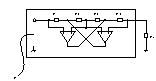
\includegraphics[width=\textwidth]{gyrator_n}
\caption{Figure~\ref{fig_gyrator} as it would appear on FidoCad for Windows.}
\label{fig_gyrator_n}
\end{figure}

An important difference from the original FidoCad\index{FidoCad} is that FidoCadJ allows to save a certain number of configuration hints in the output files. The command which is used for that is \lstinline!FJC!\index{FJC} and it should normally be placed at the very beginning of the file. The next paragraphs will describe the cases which are treated.

 \subsection{Layer setup}
 The layer setup is specified with the command \lstinline!FJC L!\index{FJC L}. FidoCadJ saves data only if the corresponding layer has been modified from its default state. The syntax is as follows:
 \begin{lstlisting}
 FJC L n xxxx yy
\end{lstlisting}
where $n$ represents the layer number (ranging from 0 to 15), $xxxx$ is a 32 bit integer containing settings about the RGB color to be used. The red component is contained in bits 16-23, the green one in bits 8-15 and the blue one in bits 0-7.
The value $yy$ is a single precision floating point constant which gives the layer transparency, comprised between 0.0 (completely transparent) and 1.0 (completely opaque).

A second important information is the name of the layer, specified (if the user has changed it) as follows:
\begin{lstlisting} 
FJC N n aaaaa
\end{lstlisting}
where $n$ is the number of the layer (integer from 0 to 15), whereas {\tt aaaa} is the name of the layer to be considered. If this command is not present, the name of the layer will be the one used by default by FidoCadJ, depending on the language and on the local configuration of the operating system.

\subsection{Electrical connection setup}
The size of the black circle used to indicate an electrical connection can be modified by the user.
When the FidoCadJ extensions are active, the selected value is saved in the file with the \lstinline!FJC C!\index{FJC C} command as follows:
\begin{lstlisting}
FJC C aaaa
\end{lstlisting}
where $aaaa$ is a double precision floating point value (positive) which gives the diameter of the electrical connection, in FidoCadJ logical units.

 \subsection{Stroke width}
 The stroke width for the ``pen'' used during the drawing of electrical schematics can be modified. FidoCadJ adopts the command \lstinline!FJC A!\index{FJC A} to specify the stroke width of the lines, ovals, B�zier, splines, rectangles and polygons. The width can be a double precision constant.
\begin{lstlisting}
FJC A aaaa
\end{lstlisting}
Where $aaaa$ represents the stroke width (in logical units). The default width is internally defined to 0.5 logical units. In older versions of FidoCadJ, a command \lstinline!FJC B bbbb!\index{FJC B} was used to specify the stroke width of curved lines (ovals, B�zier) From version 0.23.6, this differentiation has been eliminated and this command is no longer adopted.

\section{Syntax errors tolerance}

FidoCadJ is designed to tolerate errors\index{error tolerance} or
or certain syntax errors in the commands passed to the program. Obviously,
unless you have a crystal ball connected as a USB device\index{crystal ball},
the program will not be able to correct errors but it will simply
skip (and delete) all the lines involved.

An exception to this behavior is that a number of elements can
be specified without the layer, which will be considered part of the
layer\index{layer} 0 (schematics). This is for backward compatibility
with FidoCad\index{FidoCad}.


\section{Libraries format}

The file structure of a library file is quite simple:

\begin{lstlisting} 
[FIDOLIB Librairie de base]
{Syboles de base}
[000 Terminal]
LI 100 100 102 100
EV 102 98 106 102
[010 Terminal +]
LI 100 100 102 100
EV 102 98 106 102
LI 103 100 105 100
LI 104 99 104 101
[020 Terminal -]
LI 100 100 102 100
EV 102 98 106 102
LI 103 100 105 100
...
\end{lstlisting} 
The first
line contains, between square brackets\index{square brackets}, the
library's name (preceded by FIDOLIB\index{FIDOLIB}). The second line
must contain, between curly brackets, the library category under which
the macros, specified later on in the file, will be stored.

Each macro is composed by a header\index{header} (between square
brackets) and a sequence of commands. The header is constituted by
a \emph{part name} (which must be unique within the library) and its
description. The part name will be used within a FidoCadJ script, while
the description helps the user while browsing all the macros\index{macro}
contained in the file. The commands are nothing else than FidoCadJ
drawings, where the coordinate point (100,100) is used as the origin.
This is the point that will be used as the reference when the macro
will be called. In a FidoCadJ script a macro is identified by {}``library.macro''
used with the MC\index{MC} command.

Nothing prevents the calling of a macro within another macro. However,
recursion\index{recursion} (i.e. a macro that calls itself) must
be avoided.

A library \textit{must not contain} among the macro definitions any information about the FidoCadJ configuration. In other words, commands \lstinline!FJC!\index{FJC} should \textit{never} appear inside a library file.

\section{Standard Libraries}

FidoCadJ already contains two libraries traditionally supplied with
FidoCad\index{FidoCad}. In particular these are the standard library\index{standard library}
and the library that contains the PCB symbols\index{PCB library}.

However, it is possible to override the content of these two internal
library by specifying ({}``File/Options/Libraries Directory'' menu)
a directory containing the libraries to be loaded. If a file named
\lstinline!FCDstdlib.fcl! is present in this directory, its content
will be used in place of that of the standard library. If a file named
\lstinline!PCB.fcl! is present, its content will be used in place
of that of the PCB library. Other libraries having different file
names (but still with extension \lstinline!fcl!) will be loaded together
with the standard libraries.

\chapter{Conclusion} We have seen in this manual how to use FidoCadJ
to draw an electrical schematic or a simple PCB. At this stage the
reader should possess all the elements necessary to use FidoCadJ effectively
for his needs.

FidoCadJ should not be considered uniquely for the
electronics design. It can be used for any type of 2D drawing and
in many situations, provided that specific libraries are available.

The advantages of a free program is that it is completely open
to its user community. For this reason, your feedback is very
important (at least to understand if the project is worth to be developed
further, and in which direction). To contact me, you can participate to the forum of SourceForge dedicated to FidoCadJ.\footnote{\href{https://sourceforge.net/projects/fidocadj/forums/forum/997486}{https://sourceforge.net/projects/fidocadj/forums/forum/997486}}

\appendix

\chapter{Platform-specific information} \label{specifics} 


\section{MacOSX}

One of the most frequent criticisms raised against the early versions
of FidoCadJ from Macintosh users (like me, by the way) was the poor
integration of the program on MacOSX. Starting from version 0.21.1,
FidoCadJ is making specific efforts to comply better with the look
and the philosophy of Mac's native applications. For this reason,
some details in the program are slightly different when FidoCadJ is
run on an Apple platform: 
\begin{itemize}
\item by default FidoCadJ uses the Quaqua%
\footnote{\href{http://www.randelshofer.ch/quaqua/}{http://www.randelshofer.ch/quaqua/}%
}\index{Quaqua} look and feel when the complete application (FidoCadJ.app\index{FidoCadJ.app}
instead of fidocadj.jar\index{fidocadj.jar}) is run. Since Quaqua
may slow down the performance on not so recent machines, it is possible
to disable it through the settings of the Preferences menu
\item The menu bar is shown at its place, that is the top of the screen
\item The menu items {}``Preferences'' and {}``About FidoCadJ'' are
at their place, which is under the FidoCadJ menu. 
\item The program tells the operating system that it can open \lstinline!.fcd!
files; These are associated to a specific icon, which should be sufficiently
evocative.
\end{itemize}

\subsection{How to download and execute FidoCadJ on MacOSX}
FidoCadJ can work with a MacOSX\index{MacOSX} version more recent than 10.3.9 (Panther\index{Panther}).
The reason is that under the hood FidoCadJ needs at least the 1.5 version of Java, which Apple once provided with this operating system. For marketing reasons, Apple does not seem to be prone to install Java with the last versions of MacOSX\index{MacOSX}. This is an essential piece of software needed for running FidoCadJ, so you might download and install it. By the way, Apple does not allow to distribute his App Store\index{App Store} software based on Java or distributed under GPL. This is one of the most important reasons for which it is improbable that FidoCadJ will be ported to iPad\index{iPad} and iPhone\index{iPhone}.

Even if you can use directly the Java archive \lstinline!fidocad.jar! as you would do on other operating systems, on MacOSX you can use the specifically tailored application. Everything works just like a native application: you can download the disk image at the following link:

{\small
\href{http://sourceforge.net/projects/fidocadj/files/FidoCadJ_MacOSX.dmg/download}{http://sourceforge.net/projects/fidocadj/files/FidoCadJ\_ MacOSX.dmg/download}}\\
You can then open the disk image and move \lstinline!FidoCadJ.app! in the \lstinline!Applications! folder, where you can use it exactly like any other Macintosh application. To uninstall FidoCadJ, just drag  \lstinline!FidoCadJ.app! in the trash bin.


\section{Linux}
\label{installazione_linux} \textsl{by Roby IZ1CYN}\\


Prerequisite: JRE\index{JRE} 6 from Sun\index{Sun} and/or OpenJDK\index{OpenJDK}
6 JRE\index{JRE} (o previous versions compatible with the program's
specifications) must be installed. In paragraph \ref{inst_testo}
the installation of the program using only commands from a terminal
will be described. In paragraph \ref{inst_grafica}, the interaction
with a graphical environment will be used instead. A poor configuration of your Java runtime environment will determine poor performances of FidoCadJ\footnote{N.d.c. I swear, it is true! \textit{Please}, do not insult me if your favorite Linux distribution comes with an higly unreliable version of Java.}

\subsection{Using any platform, from terminal}

\label{inst_testo} Download the program using the \lstinline!wget! command:


%\lstset{language=plain,%
%	basicstyle=\tiny\ttfamily}
	
\begin{lstlisting}
$ wget http://downloads.sourceforge.net/project/fidocadj/fidocadj.jar?use_mirror=garr
--00:48:18--  http://downloads.sourceforge.net/project/fidocadj/fidocadj.jar?use_mirror=garr
           => `fidocadj.jar?use_mirror=garr'
Resolution of downloads.sourceforge.net is being done... 216.34.181.59
Connection to downloads.sourceforge.net|216.34.181.59:80... connected.
HTTP request sent, waiting for answer... 302 Found
URL: http://garr.dl.sourceforge.net/project/fidocadj/fidocadj.jar
--00:48:24--  http://garr.dl.sourceforge.net/project/fidocadj/fidocadj.jar
           => `fidocadj.jar'
Resolution of garr.dl.sourceforge.net is being done... 193.206.140.34
Connection to garr.dl.sourceforge.net|193.206.140.34:80... connected.
HTTP request sent, waiting for answer... 200 OK
Length: 343,207 (335K) [application/java-archive]

100%[====================================>] 343,207      422.48K/s             

00:48:30 (420.55 KB/s) - "fidocadj.jar" saved [343207/343207]
$
\end{lstlisting}
\lstset{
	basicstyle=\small\ttfamily}

Alternatively, or if you are experiencing problems, you can download the file from any browser from the following URL:

\href{http://sourceforge.net/projects/fidocadj/files/fidocadj.jar/download}{http://sourceforge.net/projects/fidocadj/files/fidocadj.jar/download}

and save the file in your \lstinline!/home/! directory.
	


Let's create a new directory (but at first we will become a superuser\index{superuser} by using \lstinline!su! or \lstinline!sudo -s!):

\begin{lstlisting}
# mkdir /usr/bin/fidocadj
\end{lstlisting}

\dots\ and we can move there the downloaded file (substitute \lstinline!<user>! with the user name of the account where the file has been downloaded):

\begin{lstlisting}
# mv /home/<user>/fidocadj.jar /usr/bin/fidocadj
\end{lstlisting}

Let's make the file an executable

\begin{lstlisting}
# chmod +x /usr/bin/fidocadj/fidocadj.jar
\end{lstlisting}

And we must not forget to come back to be normal users:

\begin{lstlisting}
# exit
\end{lstlisting}

And now, we can execute the program:

\begin{lstlisting}
$ /usr/bin/fidocadj/fidocadj.jar
\end{lstlisting}
%

\subsection{On a graphical system}
\label{inst_grafica}
In the example, it will be an Ubuntu\index{Ubuntu} 8.04, but things does not change so much for older or newer versions:

\begin{itemize}
\item {Let's download the file from the browser, or with Gwget or similar tools.}

\item�{We can then launch our File Manager (Nautilus, Konqueror\dots) as a root (if we do not have a specific command in the menu, we just need to launch it from the console by using \lstinline!sudo nautilus!). We can create the following directory:
\begin{lstlisting}
/usr/bin/fidocadj
\end{lstlisting}
and then move there the file we just downloaded. It will be somewhere in: 
\begin{lstlisting}
/home/<user>/
\end{lstlisting}}

\begin{figure}
\centering
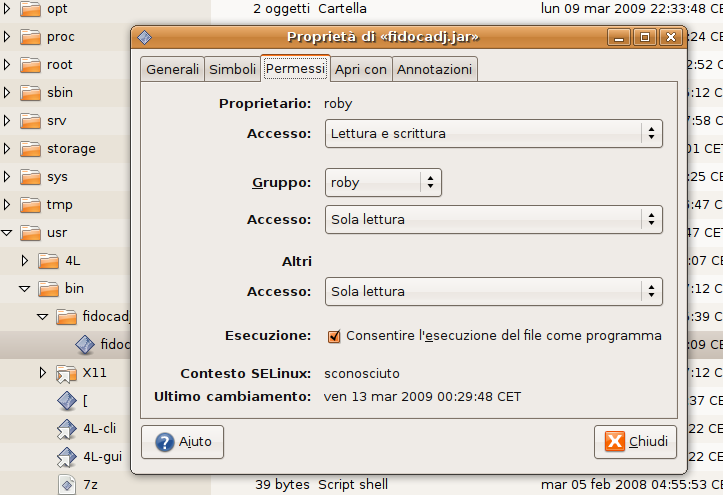
\includegraphics[width=.8\textwidth]{permessi}
\caption{The setting of file rights, on Ubuntu\index{Ubuntu} 8.04.}
\label{fig_permessi}
\end{figure}

\item {Let's do right click on the file, from the window we select the tab ``rights'', we add the check mark in front of the ``Allow the execution of the file as a program'', as shown in the figure~\ref{fig_permessi}}

\begin{figure}
\centering
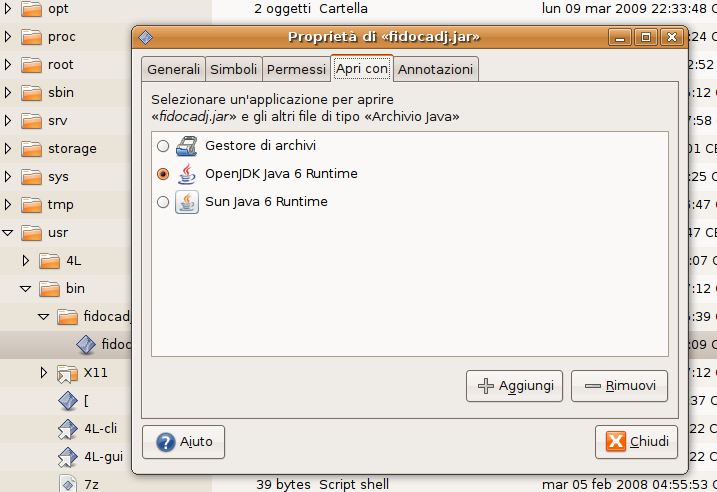
\includegraphics[width=.8\textwidth]{java6}
\caption{Set the execution with the Java virtual machine, on Ubuntu\index{Ubuntu} 8.04.}
\label{fig_java6}
\end{figure}

\item {We can select the tab ``Open as'' and select ``OpenJDK Java 6 Runtime'' or ``Sun Java 6 Runtime'', as it can be seen in figure~\ref{fig_java6}.}

\item {Let's click on ``Close'' and we are now ready to execute FidoCadJ: a double click on the executable, or we can add it to the main menu. The command to add is just \lstinline!/usr/bin/fidocadj/fidocadj.jar!.}
\end{itemize}


\section{Windows}
Since version 0.23, when FidoCadJ recognizes a Windows platform, it will try to use the native Look and Feel.

 \subsection{How to download and execute FidoCadJ}
Very often, if you have Java installed, you just have to download the  \lstinline!fidocadj.jar! file and run it with a double click. If after the download your operating system sees it as a \lstinline!zip! archive, probably Java is not available on your computer. Oracle allows to freely download and install an up to date version of the Java runtime:

\href{http://www.java.com/it/download/}{http://www.java.com/it/download/}

%\manualmark 
%\markboth{\spacedlowsmallcaps{\indexname}}% 
%{\spacedlowsmallcaps{\indexname}} 
%\refstepcounter{dummy} 
%\pagestyle{scrheadings} 
%\addcontentsline{toc}{chapter}{\tocEntry{\indexname}} 
\printindex 
\cleardoublepage
\thispagestyle{empty}
\mbox{ }
\vfill
This manual has been written using \textsc{pdf}\LaTeX\ on MacOSX.
Listings have been composed by using the  \href{http://www.ctan.org/tex-archive/macros/latex/contrib/listings/}{listings} packet. The \href{http://www.ctan.org/tex-archive/graphics/pgf/}{pgf} packet has been used for the figure~\ref{fig_schema}. All those packets are available on the CTAN archive.

%This work has been composed with the \emph{Palatino} font, by Hermann Zapf. 


\end{document}